% fix-cm: declare Computer Modern at arbitrary sizes (loaded before the
% class per its documentation) so the 56pt title page wordmark renders at
% true 56pt instead of being silently substituted at 35.83pt.
\RequirePackage{fix-cm}
\documentclass[11pt,letterpaper]{article}

% ============================================================================
% POLARIS — THE IDENTITY TOKEN SYSTEM
% Database Management Systems project report
% Author: Egor Khaklin  |  Instructor: Sami Alshalwi
% ============================================================================

% === ENCODING & TYPOGRAPHY ===
\usepackage[T1]{fontenc}
\usepackage[utf8]{inputenc}
\usepackage{textcomp}  % straight-quote glyphs for code (listings upquote)
% Latin Modern typewriter in place of cmtt: metric-compatible, but provides
% a real bold weight, so \pk{...} primary keys, heading code phrases, and
% listing keywords render genuinely bold instead of silently medium.
\renewcommand{\ttdefault}{lmtt}
\usepackage[expansion=false]{microtype}

% === MATH ===
\usepackage{amsmath}
\usepackage{amssymb}

% === PAGE GEOMETRY ===
\usepackage[
  letterpaper,
  top=0.85in,
  bottom=0.85in,
  left=1.05in,
  right=1.05in,
  headheight=13pt,
  headsep=16pt,
  footskip=28pt
]{geometry}

% === COLORS ===
\usepackage[dvipsnames,svgnames,table]{xcolor}
\definecolor{navydark}{HTML}{0C1B2E}
\definecolor{navymid}{HTML}{1B3A5C}
\definecolor{navylight}{HTML}{2D5F8A}
\definecolor{accent}{HTML}{C45B28}
\definecolor{accentlight}{HTML}{E8793F}
\definecolor{steelgray}{HTML}{4A5568}
\definecolor{tabheader}{HTML}{0F1F33}
\definecolor{tabstripe}{HTML}{F0F4F8}
\definecolor{classmark}{HTML}{8B0000}
\definecolor{gold}{HTML}{B8860B}
\definecolor{goldlight}{HTML}{D4AF37}

% === HEADERS & FOOTERS ===
\usepackage{fancyhdr}
\pagestyle{fancy}
\fancyhf{}
\renewcommand{\headrulewidth}{0.4pt}
\renewcommand{\footrulewidth}{0.2pt}
\fancyhead[L]{\small\color{steelgray}\textsc{Khaklin\,|\,Polaris}}
\fancyhead[R]{}
\fancyfoot[C]{\small\color{steelgray}Page \thepage}
\fancyfoot[R]{}

% === SECTION STYLING ===
\usepackage{titlesec}
\titleformat{\section}
  {\Large\bfseries\color{navydark}}
  {\thesection}{1em}{}
  [\vspace{-4pt}{\color{navymid}\titlerule[0.8pt]}]
\titleformat{\subsection}
  {\large\bfseries\color{navymid}}
  {\thesubsection}{0.8em}{}
\titleformat{\subsubsection}
  {\normalsize\bfseries\color{navymid}}
  {\thesubsubsection}{0.6em}{}
\titlespacing*{\section}{0pt}{13pt}{8pt}
\titlespacing*{\subsection}{0pt}{8pt}{5pt}
\titlespacing*{\subsubsection}{0pt}{6pt}{3pt}

% === TABLES ===
\usepackage{booktabs}
\usepackage{tabularx}
\usepackage{xltabular}
\usepackage[section]{placeins}  % Prevents floats from drifting past section boundaries
\usepackage{array}
\usepackage{colortbl}
\usepackage{float}
\usepackage{pdflscape}
\usepackage{ragged2e}

% === LISTS ===
\usepackage{enumitem}
\setlist[itemize]{leftmargin=1.6em, itemsep=2pt, parsep=1pt, topsep=4pt}
\setlist[itemize,1]{label=\color{accent}\textbullet}
\setlist[enumerate]{leftmargin=1.8em, itemsep=2pt, parsep=1pt, topsep=4pt}

% Prevents orphan section headers
\usepackage{needspace}

% === LINE- AND PAGE-BREAKING QUALITY ===
% Tuned tolerances instead of a global \sloppy: microtype plus a modest
% emergency stretch resolves long-identifier lines without the gaping
% interword spacing that \tolerance=9999 permits.
\tolerance=2500
\setlength{\emergencystretch}{3em}
\hbadness=2500
% Never leave a lone first/last line of a paragraph across a page break.
\clubpenalty=10000
\widowpenalty=10000
\displaywidowpenalty=10000
% With this many [H] floats and \needspace early breaks, ragged bottoms
% beat stretched interparagraph glue.
\raggedbottom

% === TIKZ ===
\usepackage{tikz}
\usetikzlibrary{positioning,arrows.meta,calc,backgrounds,fit,shapes.geometric}

% === HYPERLINKS ===
\usepackage[
  colorlinks=true,
  linkcolor=navymid,
  urlcolor=navylight,
  linktoc=all,
  hypertexnames=false,
  pdfauthor={Egor Khaklin},
  pdftitle={Polaris: The Identity Token System},
  pdfsubject={Database Management Systems project report},
  pdfkeywords={identity, post-quantum cryptography, database design, ER model, SQL},
]{hyperref}

% === CAPTION ===
\usepackage{caption}
\captionsetup{
  font={small},
  labelfont={bf,color=navymid},
  textfont={color=steelgray},
  skip=6pt
}

% === CODE LISTINGS (for SQL) ===
\usepackage{listings}
\usepackage{graphicx}
\lstset{
  basicstyle=\ttfamily\footnotesize,
  columns=fullflexible,       % natural mono spacing (no gappy fixed grid)
  keepspaces=true,            % ...while preserving hand-aligned columns
  upquote=true,               % straight quotes in SQL strings, not curly
  breaklines=true,
  breakatwhitespace=true,
  postbreak=\mbox{{\color{steelgray}\scriptsize$\hookrightarrow$}\enspace},
  frame=single,
  rulecolor=\color{navylight},
  framesep=4pt,
  backgroundcolor=\color{tabstripe},
  keywordstyle=\color{navymid}\bfseries,
  commentstyle=\color{steelgray}\itshape,
  stringstyle=\color{accent},
  showstringspaces=false,
  tabsize=2,
  numbers=left,
  numberstyle=\tiny\color{steelgray},
  numbersep=8pt,
  aboveskip=10pt plus 2pt,
  belowskip=10pt plus 2pt,
  morekeywords={RETURNING,INTERVAL,REPLACE,SERIAL}
}

% === TABLE OF CONTENTS STYLING ===
\usepackage{tocloft}
\renewcommand{\cftsecfont}{\bfseries\color{navydark}}
\renewcommand{\cftsubsecfont}{\color{navymid}}
\renewcommand{\cftsecpagefont}{\bfseries\color{navymid}}
\renewcommand{\cftsubsecpagefont}{\color{steelgray}}
\setlength{\cftbeforesecskip}{0pt}
\setlength{\cftbeforesubsecskip}{0pt}
\setcounter{tocdepth}{2}  % sections + subsections
% The TOC heading is typeset manually before \tableofcontents (and
% \contentsname is emptied), so collapse tocloft's own title spacing to
% avoid a stray gap between the rule and the first entry.
\setlength{\cftbeforetoctitleskip}{-\baselineskip}
\setlength{\cftaftertoctitleskip}{2pt}

% === CUSTOM COMMANDS ===
\newcommand{\classmark}[1]{%
  \begin{center}
    \small\scshape\color{classmark}#1
  \end{center}
}
\newcommand{\entity}[1]{\texttt{\color{navydark}#1}}
\newcommand{\pk}[1]{\underline{\textbf{\texttt{#1}}}}
\newcommand{\fk}[1]{\underline{\textit{\texttt{#1}}}}
\newcommand{\thead}[1]{\textbf{\color{white}\small #1}}

% Use case header command. \needspace{3} ensures the banner won't orphan
% at page bottom — it must keep with at least its first content row.
% The xltabular that follows handles its own page breaks for the body.
\newcommand{\usecase}[2]{%
  \needspace{3\baselineskip}%
  \vspace{6pt}%
  \noindent\colorbox{tabheader}{\parbox{\dimexpr\textwidth-2\fboxsep}{%
    \color{white}\small\bfseries\textsc{#1:} \mdseries #2}}%
  \nopagebreak[4]%
  \vspace{2pt}%
  \nopagebreak[4]%
}

% ============================================================================
\begin{document}

% Front matter: title page is unnumbered; TOC starts at i (roman).
% Body matter switches to arabic and resets to page 1 just before Section 1.

% ============================================================================
% TITLE PAGE
% ============================================================================
\begin{titlepage}
\thispagestyle{empty}

\begin{center}

% ============================================================================
% TITLE PAGE: POLARIS
%
% Design rationale (notes for future revisions):
%   The project is named after Polaris — the North Star, the celestial
%   pole of the Northern Hemisphere, fixed in the turning sky while every
%   other star revolves around it. In the schema, the ACTIVE state plays
%   the same structural role: every transition originates from or terminates
%   at it; everything else moves around it. The mythological frame and the
%   architectural principle are the same idea.
%
%   Layout: minimal text, generous whitespace. The constellation drawing
%   carries the visual weight. Three pieces of text only — name, tagline,
%   author — separated by space and a single thin gold rule. Course context
%   sits as a quiet line at the foot of the page.
% ============================================================================

\vspace*{0.9in}

% --- Subtitle (now at top) ---
{\footnotesize\scshape\color{steelgray}
The Identity Token System}

\vspace{0.65in}

% --- Project logo: Vergina sun medallion with Greek-key border ---
% Bumped from 6.12cm to 8cm — more dominant central element.
% Image is square (1:1).
\includegraphics[height=8cm]{../../site/polaris_logo_clean.png}

\vspace{0.65in}

% --- PROJECT NAME (now below logo) ---
{\fontsize{56}{60}\selectfont\scshape\color{navydark} Polaris}

\vspace{0.20in}

% --- Mythological tagline (Latin: "fixed amid the changeable") ---
{\fontsize{12}{16}\selectfont\itshape\color{navymid}
Fixus inter mutabilia}

\vspace{0.7in}

% --- Single thin gold rule, restrained ---
{\color{gold}\rule{0.85in}{0.5pt}}

\vspace{0.30in}

% --- Author ---
{\fontsize{16}{19}\selectfont\color{navydark} Egor Khaklin}

\vfill

% --- Quiet footer line ---
{\footnotesize\scshape\color{steelgray}
Seton Hill University \enspace$\cdot$\enspace Professor Sami Alshalwi}

\vspace{0.7in}

\end{center}

\end{titlepage}

% ============================================================================
% TABLE OF CONTENTS (front matter, roman numerals starting at i)
% ============================================================================
\pagenumbering{roman}
\setcounter{page}{1}
\thispagestyle{fancy}
{\color{navydark}\Large\bfseries Contents}\\[2pt]
{\color{navymid}\rule{\textwidth}{0.8pt}}
\vspace{4pt}
\renewcommand{\contentsname}{}
\tableofcontents
\newpage

% Body matter: arabic page numbers starting at 1.
\pagenumbering{arabic}
\setcounter{page}{1}

% ============================================================================
% PROJECT OVERVIEW (DOMAIN SUMMARY)
% ============================================================================
\section{Project Overview}

The database models a unified national identity infrastructure designed to replace the full set of physical and numerical credentials that Americans currently carry across different domains of life. In the present system, a single person may hold a driver's license (state DMV), a passport (federal Department of State), a Social Security card (Social Security Administration), a birth certificate (county health department), a health insurance card (private insurer), a voter registration card (state election authority), and a Real ID, each issued under different authority, with different cryptographic protections or none at all, and each creating its own identity silo. The system modeled here consolidates all of these into a single active credential per person: one physical identity token in the holder's possession at any given time, signed under a post-quantum cryptographic algorithm, and verified by authorized agencies for specific contexts.

The token is physical, durable, and quantum-resistant by design. Each individual may hold multiple provisioned tokens (a one-to-many relationship), but only one is active at any given time; the rest sit in reserve, held against the possibility of loss, damage, or compromise of the active token. If the active token is lost, a reserve token can be activated through an expedited process rather than requiring full reissuance from scratch. A previously active token transitions to dormant status when superseded and is retained for audit. The cryptographic algorithm entity is populated with real post-quantum standards (ML-DSA, SLH-DSA) alongside legacy classical algorithms (ECDSA, RSA) so that queries can distinguish quantum-resistant from deprecated signing material directly in SQL.

Digital projection extends the physical token into the holder's personal devices without introducing cloud storage. A token may authorize bindings on a small number of personal devices (phone, tablet, watch), each of which stores a cryptographic copy in the device's secure enclave and can present the credential in contexts that accept digital presentation. The physical token remains authoritative; device bindings are derivative and independently revocable. No backup credential is ever stored on a server, and no cloud provider holds any part of the token. If a device is lost, its binding can be revoked without affecting the physical token or other device bindings.

Context-scoped verification is the key architectural feature. A single token supports verification for banking, employment, healthcare, travel, voting, motor vehicle operation, and government benefits, but each verification event occurs in exactly one context. The verification context entity carries the minimum security level and biometric requirement per context, and a permission junction determines which contexts a given token is authorized for. A token authorized only for banking and employment cannot be used at a TSA checkpoint; a token authorized only for motor vehicle operation cannot be presented as a passport. The verification layer is where the system generates volume. Every time a bank, employer, hospital, airport, polling station, or government agency verifies someone's identity, a verification event record is created capturing who verified, when, for what context, and with what outcome. This is the transactional core of the database and the source of the most interesting queries.

Two privacy and security features distinguish this design from a naive centralized identity database. First, \textbf{zero-knowledge verification} allows most verification events to record that a valid token was presented without recording which token. The \texttt{disclosure\_level} column on each verification event controls what is stored: \texttt{ZERO\_KNOWLEDGE} (no token identity, only a cryptographic commitment), \texttt{SELECTIVE} (specific attributes disclosed, e.g., age or citizenship but not address), or \texttt{FULL} (complete token identity, used only under warrant or with explicit consent). This prevents the verification log from functioning as a comprehensive surveillance database while preserving audit capability for fraud and abuse. Second, \textbf{on-device biometric binding} ties each token to its holder through a local biometric check performed by the token hardware itself. The biometric template never leaves the device and is never stored in the database; \entity{IdentityToken} records only the binding type (\texttt{FINGERPRINT}, \texttt{FACE}, \texttt{IRIS}, or \texttt{NONE}), enrollment date, witnessing agency, and liveness-check method used at enrollment. If the token is lost, the biometric template is destroyed with it.

\subsection{Why Post-Quantum from Day One}
\label{subsec:pq-day-one}

The decision to model post-quantum signing as a first-class property of the schema, rather than as a migration target for a later revision, follows from the time horizon of identity data. Most cryptographically protected information has a finite secrecy horizon: a session key for a session, a transaction for a settlement window, an industrial design for a product cycle. Identity data does not. A name, date of birth, citizenship, biometric binding, and any genomic anchor carry a horizon equal to the holder's lifetime plus the lifetimes of relatives whose genome partially recovers from theirs. The information is multi-generational, and once exposed cannot be rotated, revoked, or reissued.

Mosca's inequality (Mosca, 2018) formalizes the resulting risk. Let $X$ be the secrecy horizon, $Y$ the migration time, and $Z$ the time until a cryptographically relevant quantum computer enters service: if $X + Y > Z$, migration is already behind schedule. For identity records built on biometric or genomic anchors, $X$ falls in the 90--120-year range; for a national-scale infrastructure $Y$ is on the order of a decade; by every public estimate $Z$ is shrinking faster than projected. The inequality is not a future condition but the present one: adversaries running harvest-now-decrypt-later programs are not waiting to attack identity data, they are waiting for the rendering event at which the protection dissolves on its own. A credential system deployed on classical cryptography in 2026 is therefore not a working system requiring future migration; it is a deferred compromise, and the schema is designed accordingly. \entity{CryptographicAlgorithm} is modeled as a queryable entity with \texttt{quantum\_resistant} and \texttt{deprecation\_date} columns; \entity{AgencyAlgorithmAuth} bounds which agencies may issue under which algorithms; \texttt{predecessor\_token\_id} chains cryptographic generations forward across reissuance; classical algorithms appear in the schema only to make their deprecation queryable, while new tokens are issued exclusively under post-quantum primitives (ML-DSA, SLH-DSA) per the FIPS 203/204/205 finalization of August 2024.

\subsection{Scope at a Glance}

\begin{itemize}
  \item \textbf{Ten entities on the ER diagram} (Individual, Agency, CryptographicAlgorithm, VerificationContext, IdentityToken, TokenLifecycleEvent, VerificationEvent, DeviceBinding, BlockchainAnchor, RevocationList) plus \textbf{two junction tables} (AgencyAlgorithmAuth, TokenPermission) to resolve the M:N relationships.
  \item \textbf{One active credential per person} (\textsc{Holds} is 1:N with a uniqueness constraint). Each person may have multiple tokens provisioned, but only one may be \texttt{ACTIVE} at a time. Additional tokens sit in \texttt{RESERVE} state for emergency activation; superseded tokens transition to \texttt{DORMANT} and are retained for audit.
  \item \textbf{Two one-to-many relationships into IdentityToken} (from Agency as issuer, from CryptographicAlgorithm as signer) and two outward from it (to TokenLifecycleEvent via \textsc{Generates}, to VerificationEvent via \textsc{Verified}).
  \item \textbf{Two many-to-many relationships} (Agency$\leftrightarrow$CryptographicAlgorithm via \textsc{Authorized}, IdentityToken$\leftrightarrow$VerificationContext via \textsc{Permitted}) each resolved through a dedicated junction table with its own attributes.
  \item \textbf{One high-volume associative entity} (VerificationEvent) recording every verification transaction: which token was verified, by which agency, for what context, with what outcome.
  \item \textbf{Domain constraints} enforced through \texttt{CHECK} clauses on status fields to prevent invalid values, and through a partial unique index to enforce one-active-token-per-person.
\end{itemize}

\textit{Scope note:} DeviceBinding, BlockchainAnchor, and RevocationList are included as first-class entities because each represents real verifier-facing data that a production system would need to query: on-device digital projections (DeviceBinding), decentralized-identifier anchoring for the alternative trust architecture noted in Limitations (BlockchainAnchor), and verifier-facing historical revocation records for audit-accurate freshness checks (RevocationList). Together they remain within conceptual ER scope as entities directly subsidiary to IdentityToken rather than as implementation details deferred to the relational model.

\subsection{Reading Guide}
\label{subsec:reading-guide}

The body of this report follows the standard database-design pipeline. Section~\ref{sec:info-collection} collects the operational requirements through user roles and seven concrete use cases. Section~\ref{sec:db-requirements} restates those requirements as numbered functional and non-functional specifications. Sections~\ref{sec:info-analysis} through~\ref{sec:rel-algebra} then trace the design forward through the standard sequence: information analysis identifies the entities and relationships, ER modeling formalizes them in Chen notation, relational mapping derives the schema (with a normalization proof in~\ref{subsec:normalization} establishing that every relation is in BCNF), SQL implementation realizes it, and relational algebra expresses representative queries. Each stage is the input to the next, and the use cases introduced at the start are referenced at every subsequent stage so that the operational pattern and the schema-level construct that supports it can be read against each other.

The appendices are not afterthoughts. They are the dimensions in which the body's claims are tested. Appendix~\ref{app:state-machine} formalizes the lifecycle invariants that the schema's \texttt{CHECK} constraints alone cannot express. Appendix~\ref{app:indexing} addresses the query-plan and partitioning concerns that determine whether the schema can carry national-scale verification volume. Appendix~\ref{app:comparison} situates the design against a federated national eID, Aadhaar, mDL, EU eIDAS 2.0, and the W3C verifiable-credentials stack, locating the distinguishing feature (\texttt{disclosure\_level} as a schema-level mechanism) against five existing approaches. Appendix~\ref{app:threat-model} runs the schema through STRIDE and names the three threats the database layer cannot mitigate. Appendix~\ref{app:substrate} formalizes the deeper architectural argument: cryptographic primitives are the substrate of digital sovereignty, and every higher-level property is derivative of them. Appendix~\ref{app:beyond-biometric} sketches the two horizons beyond fingerprint-, face-, and iris-binding (genomic and quantum-observer) and the schema extensions each would require.

A reader evaluating the database deliverable can read sections~\ref{sec:info-collection} through~\ref{sec:rel-algebra} and Appendices~\ref{app:state-machine} and~\ref{app:indexing}; a reader evaluating the architectural argument should add Appendices~\ref{app:comparison} through~\ref{app:beyond-biometric}.

% ============================================================================
% STEP 1: INFORMATION COLLECTION
% ============================================================================
% \newpage  -- removed; let section flow naturally
\section{Information Collection}
\label{sec:info-collection}

\subsection{Problem Domain}

The chosen problem domain is \textbf{national identity credentialing}. The current US system distributes identity authority across federal, state, county, and private issuers, with each credential carrying a different cryptographic posture (or none), serving a different verification context, and creating its own identity silo. The system specified here consolidates all civic identity into a single quantum-resistant hardware token per individual while preserving the federation of issuing authorities and the per-context verification model already in operation.

Information was gathered through analysis of: (1) current US credential issuance practices across federal, state, and county agencies; (2) NIST post-quantum cryptography standards (FIPS 203 for key encapsulation, FIPS 204 for digital signatures based on ML-DSA, FIPS 205 for stateless hash-based signatures based on SLH-DSA), finalized August 2024; (3) zero-knowledge proof literature, including the disclosure-level taxonomy used in selective-disclosure verifiable credentials; (4) the W3C Decentralized Identifier specification for the optional ledger-anchoring path; and (5) failure-mode analysis of relevant historical incidents (the 2017 Equifax breach as a case study in centralized identity-data concentration; the 2020 SolarWinds compromise as a case study in supply-chain risk to issuing authorities; historical denaturalization programs as a case study in issuer-discretion abuse).

\needspace{3\baselineskip}
\subsection{User Roles}

Five user roles interact with the database. Each has a distinct access pattern, summarized below.

\begin{table}[H]
\centering
\footnotesize
\caption{User roles and their database access patterns.}
\setlength{\tabcolsep}{5pt}
\renewcommand{\arraystretch}{1.1}
\rowcolors{2}{tabstripe}{white}
\begin{tabularx}{\textwidth}{>{\bfseries\RaggedRight\arraybackslash}p{1.85in} >{\RaggedRight\arraybackslash}X}
\toprule
\rowcolor{tabheader}
\thead{Role} & \thead{Description and Database Access Pattern} \\
\midrule
Individual (Token Holder) & The natural person enrolled in the system. Does not directly write to the database. Indirectly triggers \entity{VerificationEvent} inserts whenever they present a token at a verifier and triggers \entity{DeviceBinding} inserts when they bind a personal device. May initiate reserve activation through an issuing agency. \\
Issuing Agency Personnel & Authorized staff at federal, state, county, or private issuing authorities. Inserts into \entity{Individual} (during initial enrollment) and \entity{IdentityToken}; writes to \entity{TokenLifecycleEvent} on every state change; writes to \entity{RevocationList} when revoking. Subject to the agency's authorization level and \entity{AgencyAlgorithmAuth} entries. \\
Verifying Agency Personnel & Authorized staff or automated systems at any verifier (banks, hospitals, airports, polling stations, employers, government benefit offices). Reads from \entity{IdentityToken} and \entity{TokenPermission} to validate; writes a single \entity{VerificationEvent} record per verification at the appropriate \texttt{disclosure\_level}. Cannot modify token state. \\
System Administrator & Manages the schema itself, the \entity{CryptographicAlgorithm} table, and \entity{AgencyAlgorithmAuth} authorization grants. Identifies tokens at risk from algorithm deprecation and orchestrates migration cohorts. Has read access across all tables for operational monitoring. \\
Audit / Court Official & Subject to a warrant or explicit holder consent. Reads from \entity{VerificationEvent}, \entity{TokenLifecycleEvent}, and \entity{RevocationList} to reconstruct a token's history for fraud investigation, abuse review, or constitutional challenge. Can only view \texttt{FULL} disclosure-level events without further authorization; \texttt{ZERO\_KNOWLEDGE} events return no identifying information by design. \\
\bottomrule
\end{tabularx}
\end{table}

\subsection{Use Cases}

The seven use cases below describe how each role interacts with the database during a typical operational year. They cover the full token lifecycle (issuance, activation, verification, device binding, replacement, revocation) and the two cross-cutting administrative concerns (algorithm migration, warrant-authorized audit). Each use case names the database tables touched, the operations performed, and the resulting state changes.

Each entry follows the same structure: \textbf{Primary Actor} (the role that initiates the operation), \textbf{Secondary Actor} (the role or component that participates passively), \textbf{Goal} (the post-condition the operation aims to establish), \textbf{Trigger} (the event that initiates the use case), \textbf{Main Flow} (the ordered sequence of database operations), \textbf{Tables Touched} (the schema surface the operation exercises), and a \textbf{Note} field where a constraint or implementation detail deserves explicit mention. The sequence below moves from initial enrollment (UC-1) through the two verification contexts that exercise the disclosure model (UC-2 zero-knowledge, UC-3 full disclosure), into exception handling (UC-4 reserve activation, UC-5 device binding), and concludes with the two administrative use cases (UC-6 algorithm migration, UC-7 warrant-authorized audit) that justify several of the schema's less obvious design decisions.

\usecase{UC-1}{New Token Issuance and Initial Activation}
\noindent\begin{xltabular}{\textwidth}{>{\bfseries}p{1.4in} >{\RaggedRight\arraybackslash}X}
Primary Actor & Issuing Agency Personnel \\
Secondary Actor & Individual (citizen presenting for enrollment) \\
Goal & Create a new identity token, bind it to an individual under a quantum-resistant algorithm, and place it in \texttt{ACTIVE} state. \\
Trigger & A citizen presents identity-establishing documents at an authorized issuing agency for the first time, or for re-enrollment following revocation. \\
Main Flow &
\begin{enumerate}
  \item Issuing officer validates that their agency holds an \texttt{ISSUE} or \texttt{BOTH} grant in \entity{AgencyAlgorithmAuth} for the chosen algorithm.
  \item If the individual has no existing record, \texttt{INSERT} a new row into \entity{Individual}.
  \item \texttt{INSERT} a new row into \entity{IdentityToken} with \texttt{status='RESERVE'}, populated FK references to \entity{Individual}, \entity{Agency}, and \entity{CryptographicAlgorithm}.
  \item \texttt{INSERT} a \entity{TokenLifecycleEvent} of type \texttt{ISSUED}.
  \item Hardware binding ceremony: officer witnesses biometric enrollment on the token's secure enclave; \texttt{UPDATE} the token's biometric metadata fields and \texttt{enrollment\_witness\_agency\_id}.
  \item \texttt{UPDATE} \entity{IdentityToken} setting \texttt{status='ACTIVE'} and \texttt{activated\_date}; the partial unique index enforces no other active token exists for this individual.
  \item \texttt{INSERT} a \entity{TokenLifecycleEvent} of type \texttt{ACTIVATED}.
  \item \texttt{INSERT} default \entity{TokenPermission} rows for the contexts the holder is eligible for.
\end{enumerate} \\
Tables Touched & \entity{Individual}, \entity{IdentityToken}, \entity{TokenLifecycleEvent}, \entity{TokenPermission}, \entity{AgencyAlgorithmAuth} (read-only check) \\
\end{xltabular}

\usecase{UC-2}{Banking Verification (Zero-Knowledge)}
\noindent\begin{xltabular}{\textwidth}{>{\bfseries}p{1.4in} >{\RaggedRight\arraybackslash}X}
Primary Actor & Verifying Agency Personnel (bank, automated kiosk, or online banking system) \\
Secondary Actor & Individual presenting their token \\
Goal & Confirm the holder presents a valid token authorized for \texttt{BANKING} without recording the token's identity in the verification log. \\
Trigger & A customer initiates a transaction or account-access action that requires identity attestation. \\
Main Flow &
\begin{enumerate}
  \item Verifier system reads \entity{IdentityToken} to confirm \texttt{status='ACTIVE'} and the signing \entity{CryptographicAlgorithm} is not deprecated.
  \item Verifier system checks \entity{TokenPermission} for an entry where \texttt{context\_id} corresponds to \texttt{BANKING} and \texttt{permission\_level} is sufficient.
  \item Token hardware produces a zero-knowledge proof of validity that does not reveal \texttt{token\_id}; the proof commitment is stored in \texttt{proof\_commitment}.
  \item \texttt{INSERT} a \entity{VerificationEvent} with \texttt{token\_id=NULL}, \texttt{disclosure\_level='ZERO\_KNOWLEDGE'}, and the cryptographic commitment retained for fraud-investigation correlation.
\end{enumerate} \\
Tables Touched & \entity{IdentityToken} (read), \entity{TokenPermission} (read), \entity{VerificationEvent} (insert), \entity{VerificationContext} (read) \\
\end{xltabular}

\usecase{UC-3}{Travel Verification at TSA / Border Crossing (Full Disclosure)}
\noindent\begin{xltabular}{\textwidth}{>{\bfseries}p{1.4in} >{\RaggedRight\arraybackslash}X}
Primary Actor & Verifying Agency Personnel (TSA officer, CBP agent) \\
Secondary Actor & Individual presenting their token at a security checkpoint \\
Goal & Confirm the holder's full identity for a context that legally requires identification under federal authority. \\
Trigger & The holder presents at a designated travel checkpoint where federal law authorizes full identity verification. \\
Main Flow &
\begin{enumerate}
  \item Verifier system reads \entity{IdentityToken} to confirm \texttt{status='ACTIVE'} and biometric binding is appropriate to context (\texttt{TRAVEL} requires biometric per \entity{VerificationContext}).
  \item Token hardware performs a liveness-checked biometric match locally; result is binary, no template leaves the device.
  \item Verifier system checks \entity{TokenPermission} for \texttt{TRAVEL} authorization.
  \item \texttt{INSERT} a \entity{VerificationEvent} with full \texttt{token\_id} reference, \texttt{disclosure\_level='FULL'}, and the verifier's location captured in \texttt{requestor\_location}.
\end{enumerate} \\
Tables Touched & \entity{IdentityToken} (read), \entity{TokenPermission} (read), \entity{VerificationContext} (read), \entity{VerificationEvent} (insert) \\
\end{xltabular}

\usecase{UC-4}{Reserve Token Activation After Loss}
\noindent\begin{xltabular}{\textwidth}{>{\bfseries}p{1.4in} >{\RaggedRight\arraybackslash}X}
Primary Actor & Issuing Agency Personnel \\
Secondary Actor & Individual reporting loss of their active token \\
Goal & Revoke the lost token and promote a pre-provisioned reserve to \texttt{ACTIVE} without requiring full reissuance from scratch. \\
Trigger & The holder reports loss, theft, damage, or compromise of their active token to an authorized issuing agency. \\
Main Flow &
\begin{enumerate}
  \item Officer authenticates the individual through alternative means (in-person identification, secondary biometric, sworn statement).
  \item \texttt{UPDATE} the lost token's \entity{IdentityToken} record setting \texttt{status='LOST'} or \texttt{'REVOKED'}.
  \item \texttt{INSERT} a \entity{RevocationList} record with appropriate \texttt{reason\_code} (\texttt{LOST}, \texttt{STOLEN}, \texttt{COMPROMISED}) and a \texttt{published\_location} URL.
  \item \texttt{INSERT} a \entity{TokenLifecycleEvent} of type \texttt{LOST} or \texttt{REVOKED}.
  \item Select an existing \entity{IdentityToken} for the same individual where \texttt{status='RESERVE'}.
  \item \texttt{UPDATE} the reserve token: set \texttt{status='ACTIVE'}, populate \texttt{predecessor\_token\_id} with the lost token's \texttt{token\_id}, increment \texttt{activation\_sequence}, set \texttt{activated\_date}.
  \item \texttt{INSERT} a \entity{TokenLifecycleEvent} of type \texttt{ACTIVATED} on the new active token.
\end{enumerate} \\
Tables Touched & \entity{IdentityToken} (update), \entity{RevocationList} (insert), \entity{TokenLifecycleEvent} (insert) \\
Note & The partial unique index on \texttt{(individual\_id) WHERE status='ACTIVE'} permits both the \texttt{RESERVE} insert (step 3) and the \texttt{ACTIVE} update (step 6) within a single transaction: at step 3 the new row has status \texttt{RESERVE} (outside the partial-index predicate, no uniqueness check); at step 6 the row transitions into the predicate and the uniqueness check fires only then, when the holder has no other active token. \\
\end{xltabular}

\usecase{UC-5}{Device Binding (Digital Projection to a Personal Device)}
\noindent\begin{xltabular}{\textwidth}{>{\bfseries}p{1.4in} >{\RaggedRight\arraybackslash}X}
Primary Actor & Individual \\
Secondary Actor & The personal device's secure enclave (cryptographic counterparty) \\
Goal & Authorize a personal phone, tablet, or watch to present the token in contexts that accept digital presentation, without storing any credential material in the cloud. \\
Trigger & The holder initiates device-binding from their physical token through a tap-to-pair or NFC handshake. \\
Main Flow &
\begin{enumerate}
  \item Token hardware generates a device-specific cryptographic projection bound to the device's secure-enclave fingerprint.
  \item \texttt{INSERT} into \entity{DeviceBinding} with \texttt{token\_id}, \texttt{device\_type}, the secure-enclave-attested \texttt{device\_fingerprint}, the \texttt{binding\_method} (\texttt{SECURE\_ENCLAVE}, \texttt{TITAN\_SECURITY}, etc.), and an \texttt{expires\_date}.
  \item \texttt{INSERT} a \entity{TokenLifecycleEvent} of type \texttt{DEVICE\_BOUND}.
\end{enumerate} \\
Reverse Flow (revocation) & On device loss, \texttt{UPDATE} the binding to \texttt{status='REVOKED'} with a \texttt{revocation\_reason} and \texttt{INSERT} a \texttt{DEVICE\_REVOKED} lifecycle event. The physical token and other device bindings are unaffected. \\
Tables Touched & \entity{DeviceBinding} (insert/update), \entity{TokenLifecycleEvent} (insert) \\
\end{xltabular}

\usecase{UC-6}{Algorithm Migration Audit}
\noindent\begin{xltabular}{\textwidth}{>{\bfseries}p{1.4in} >{\RaggedRight\arraybackslash}X}
Primary Actor & System Administrator \\
Goal & Identify the cohort of tokens whose signing algorithm is approaching deprecation so that a coordinated reissuance effort can be scheduled before the deprecation date passes. \\
Trigger & A scheduled quarterly review, or an emergency NIST advisory shortening an algorithm's deprecation window. \\
Main Flow &
\begin{enumerate}
  \item Run a join query against \entity{IdentityToken}, \entity{Individual}, and \entity{CryptographicAlgorithm} filtered by \texttt{status='ACTIVE'} and a \texttt{deprecation\_date} within the operational horizon (typically 24 months).
  \item Group results by \texttt{issuing\_agency\_id} to allocate reissuance load to the agencies that must perform it.
  \item Output is a worklist of (token, holder, current algorithm, target algorithm) tuples that drives the reissuance schedule.
\end{enumerate} \\
Tables Touched & \entity{IdentityToken} (read), \entity{Individual} (read), \entity{CryptographicAlgorithm} (read), \entity{Agency} (read) \\
Note & Reissuance itself is implemented as UC-1 followed by UC-4 (lost-token flow) for each affected token, with \texttt{predecessor\_token\_id} chaining the cryptographic generations. \\
\end{xltabular}

\usecase{UC-7}{Warrant-Authorized Verification History Review}
\noindent\begin{xltabular}{\textwidth}{>{\bfseries}p{1.4in} >{\RaggedRight\arraybackslash}X}
Primary Actor & Audit / Court Official \\
Secondary Actor & The token holder under investigation \\
Goal & Reconstruct a token's verification history under valid legal authority, returning only the records the disclosure model permits. \\
Trigger & A court-issued warrant naming a specific \texttt{individual\_id}, presented through the audit interface. \\
Main Flow &
\begin{enumerate}
  \item Auditor presents warrant credentials; the audit interface validates the warrant scope (specific individual, specific time window, specific context if narrowed).
  \item Run a join query against \entity{VerificationEvent}, \entity{IdentityToken}, \entity{Individual}, and \entity{VerificationContext} filtered by the warrant's parameters.
  \item Apply the disclosure filter: events with \texttt{disclosure\_level='ZERO\_KNOWLEDGE'} return no token-identifying data and are tallied only as aggregate counts; \texttt{SELECTIVE} events return the disclosed attributes; \texttt{FULL} events return complete records.
  \item Augment the result with the corresponding \entity{TokenLifecycleEvent} and \entity{RevocationList} entries to produce a complete history.
\end{enumerate} \\
Tables Touched & \entity{VerificationEvent}, \entity{TokenLifecycleEvent}, \entity{RevocationList}, \entity{IdentityToken}, \entity{Individual}, \entity{VerificationContext} (all read) \\
Note & The disclosure model is the architectural protection against the verification log functioning as a comprehensive surveillance database. The schema permits the warrant query; the disclosure level governs what the warrant query can return. \\
\end{xltabular}

\vspace{6pt}
These seven use cases collectively exercise ten of the schema's twelve tables and the principal relationships among them. \entity{AgencyAlgorithmAuth} is read by UC-1 as an authorization gate but is not written by any use case (entries are populated administratively rather than as a side effect of issuance or verification); \entity{BlockchainAnchor} is exercised at the SQL layer rather than through the operational use cases above, since the optional DID-anchoring path is implementer-driven rather than user-driven. The sections that follow specify the database requirements, analyze the entities and relationships in detail, formalize them in a Chen-notation ER diagram, map them to a relational schema, implement them in SQL, and express representative queries from these use cases in relational algebra.

\needspace{3\baselineskip}
\subsection{Use-Case Coverage Matrix}

The matrix below shows which tables each use case reads from (\textsc{R}) and writes to (\textsc{W}). The pattern verifies that every table appears in at least one use case and that every use case touches at least two tables. The schema is neither under-utilized nor over-fragmented.

\begin{table}[H]
\centering
\footnotesize
\caption{Use cases mapped to tables (R = read, W = write).}
\rowcolors{2}{tabstripe}{white}
\renewcommand{\arraystretch}{1.05}
\begin{tabularx}{\textwidth}{>{\bfseries}p{0.45in} *{8}{>{\centering\arraybackslash}X} >{\centering\arraybackslash}p{0.5in}}
\toprule
\rowcolor{tabheader}
\thead{} & \thead{Indv.} & \thead{Agcy.} & \thead{Alg.} & \thead{Tok.} & \thead{TLE} & \thead{VE} & \thead{Ctx.} & \thead{Perm.} & \thead{Other} \\
\midrule
UC-1 & W & R & R & W & W & --- & --- & W & --- \\
UC-2 & --- & R & --- & R & --- & W & R & R & --- \\
UC-3 & --- & R & --- & R & --- & W & R & R & --- \\
UC-4 & --- & --- & --- & W & W & --- & --- & --- & RevList (W) \\
UC-5 & --- & --- & --- & R & W & --- & --- & --- & DevBind (W) \\
UC-6 & R & R & R & R & --- & --- & --- & --- & --- \\
UC-7 & R & --- & --- & R & R & R & R & --- & RevList (R) \\
\bottomrule
\end{tabularx}
\end{table}

\entity{IdentityToken} appears in all seven use cases, confirming its role as the architectural hub. \entity{Agency} (read in four cases as either issuer, verifier, witness, or actor) and \entity{TokenLifecycleEvent} (written in four cases as the audit-trail backbone) follow at the next tier. \entity{VerificationEvent} dominates the verification-context use cases (UC-2 and UC-3) and is the high-volume transactional table. The pattern of writes reveals two entry points to the schema: enrollment (UC-1) and verification (UC-2, UC-3); everything else is downstream lifecycle administration. The read/write asymmetry sorts the use cases into three load profiles the schema must satisfy under production traffic: read-heavy, low-latency verification (UC-2, UC-3, producing one append-only row each); write-heavy issuance (UC-1, writing to four tables in a single transaction); and read-only audit (UC-7, reconstructing narratives across six tables without modifying any).


% ============================================================================
% STEP 2: DATABASE REQUIREMENTS DOCUMENT
% ============================================================================
% \newpage  -- removed; let section flow naturally
\section{Database Requirements Document}
\label{sec:db-requirements}

\subsection{Project Scope}
The \textit{Identity Token System} is a unified national identity infrastructure designed to replace the current fragmented set of physical and digital credentials (driver's licenses, passports, Social Security cards, birth certificates, Real ID, voter registration cards, health insurance cards) with a single quantum-resistant hardware token per citizen. The system supports context-scoped verification across agencies and jurisdictions while preserving strong privacy guarantees through zero-knowledge and selective disclosure mechanisms. The relational database specified in this report is the persistent backbone of that infrastructure: it stores the issuance, lifecycle, authorization, and verification records that make federated trust auditable while keeping biometric templates and unnecessary verification metadata out of the database entirely.

\subsection{Functional Requirements}

\begin{itemize}
  \item One active credential per person, with reserve tokens for redundancy and expedited recovery (FR-1).
  \item Context-scoped verification (\texttt{BANKING}, \texttt{EMPLOYMENT}, \texttt{HEALTHCARE}, \texttt{TRAVEL}, \texttt{VOTING}, \texttt{MOTOR\_VEHICLE}, \texttt{GOVERNMENT\_BENEFITS}) with per-context biometric and security-level requirements (FR-2).
  \item Zero-knowledge verification (\texttt{ZERO\_KNOWLEDGE}, \texttt{SELECTIVE}, \texttt{FULL} disclosure levels) to prevent the verification log from becoming a surveillance database (FR-3).
  \item On-device biometric binding (\texttt{FINGERPRINT}, \texttt{FACE}, \texttt{IRIS}, \texttt{NONE}) with no biometric templates stored centrally (FR-4).
  \item Full append-only audit trail via \entity{TokenLifecycleEvent} and \entity{VerificationEvent} (FR-5).
  \item Optional post-quantum decentralized-identifier (DID) anchoring on distributed ledgers (FR-6).
  \item Agency authorization matrix controlling which agencies may issue or verify under each cryptographic algorithm (FR-7).
  \item Token succession tracking through a self-referential \texttt{predecessor\_token\_id} foreign key, capturing the cryptographic lineage when a reserve is activated or a token is reissued (FR-8).
  \item Verifier-facing revocation publication, distinct from the token's own status field, to support audit-accurate freshness checks (FR-9).
\end{itemize}

\subsection{Non-Functional Requirements}

\begin{itemize}
  \item Quantum resistance using ML-DSA and SLH-DSA (NIST FIPS 204 and 205 post-quantum standards) as primary signature algorithms; legacy classical algorithms (ECDSA, RSA) retained only for queryable deprecation tracking (NFR-1).
  \item High-volume transactional support: the verification layer must accept thousands of \entity{VerificationEvent} inserts per day per major verifier without locking contention (NFR-2).
  \item Strict referential integrity enforced through foreign keys on every cross-entity reference; \texttt{CHECK} constraints on every enumerated field; partial uniqueness on the active-token invariant (NFR-3).
  \item Auditability: every token state transition produces a \entity{TokenLifecycleEvent}; the lifecycle table is append-only by convention and tooling, not by storage engine (NFR-4).
  \item Support for token lifecycle states (\texttt{ACTIVE}, \texttt{RESERVE}, \texttt{DORMANT}, \texttt{REVOKED}, \texttt{LOST}, \texttt{EXPIRED}) with constrained transitions enforced at the application layer (NFR-5).
  \item Privacy-preserving by construction: no biometric template, no verification location more granular than necessary, and no token identity stored on \texttt{ZERO\_KNOWLEDGE} verification events (NFR-6).
\end{itemize}

% ============================================================================
% STEP 3: INFORMATION ANALYSIS
% ============================================================================
% \newpage  -- removed; let section flow naturally
\section{Information Analysis}
\label{sec:info-analysis}

This section identifies the entities, relationships, and key constraints that the requirements imply, before formalizing them as an ER diagram in the next section. The analysis distinguishes \textit{conceptual} entities (independent things the database represents) from \textit{associative} entities (records that exist only because two other entities relate to each other) and notes the constraints that must be carried forward into the schema.

\needspace{3\baselineskip}
\subsection{Entity Identification}
\label{subsec:entity-id}

Ten entities emerge from the requirements. They divide cleanly into three groups: \textbf{principals} (the actors and authorities), \textbf{the central artifact} (the token itself), and \textbf{records} (the events and subsidiary structures that exist relative to a token).

\begin{table}[H]
\centering
\footnotesize
\caption{Entities identified during requirements analysis.}
\rowcolors{2}{tabstripe}{white}
\begin{tabularx}{\textwidth}{>{\bfseries}p{1.7in} l >{\RaggedRight\arraybackslash}X}
\toprule
\rowcolor{tabheader}
\thead{Entity} & \thead{Group} & \thead{Why It Exists} \\
\midrule
Individual & Principal & The natural person whom the token credentials. \\
Agency & Principal & The federal, state, county, or private authority that issues or verifies. \\
CryptographicAlgorithm & Principal & The signing primitive used by tokens; modeled as a first-class entity so deprecation and quantum-resistance status are queryable. \\
VerificationContext & Principal & The seven fixed contexts in which verification can occur; modeled as an entity rather than an enum so per-context security and biometric requirements can be queried and joined. \\
\midrule
IdentityToken & Central artifact & The credential itself; every other relationship in the schema either originates from or terminates at this entity. \\
\midrule
TokenLifecycleEvent & Record & Append-only log of state transitions on a single token. \\
VerificationEvent & Record & The high-volume transactional record produced every time a token is presented for verification. \\
DeviceBinding & Record & A digital projection of a physical token to a personal device's secure enclave. \\
BlockchainAnchor & Record & The optional ledger-anchored DID commitment for the alternative trust architecture. \\
RevocationList & Record & Verifier-facing historical record of revocations, separating revocation publication from token status. \\
\bottomrule
\end{tabularx}
\end{table}

\subsection{Relationship Identification}
\label{subsec:relationship-id}

Thirteen relationships connect these ten entities, including one self-referential link on \entity{IdentityToken}. The pattern is hub-and-spoke: \entity{IdentityToken} is the hub, and most other entities relate to it directly. The single peer-to-peer relationship is \entity{Agency}~\textsc{Authorized}~\entity{CryptographicAlgorithm}, the authorization matrix that governs which agencies may use which signing algorithms.

\begin{itemize}
  \item \textbf{1:N relationships into \entity{IdentityToken}} from \entity{Individual} (\textsc{Holds}), \entity{Agency} (\textsc{Issues}), and \entity{CryptographicAlgorithm} (\textsc{Signs}).
  \item \textbf{1:N relationships out of \entity{IdentityToken}} to \entity{TokenLifecycleEvent} (\textsc{Generates}), \entity{VerificationEvent} (\textsc{Verified}), \entity{DeviceBinding} (\textsc{Projects\_To}), and \entity{RevocationList} (\textsc{Revoked\_Via}).
  \item \textbf{0..1:1 relationship} from \entity{IdentityToken} to \entity{BlockchainAnchor} (\textsc{Anchored\_To}), optional on the token side: a token may have zero or one anchor; an anchor always references exactly one token.
  \item \textbf{M:N relationship} between \entity{Agency} and \entity{CryptographicAlgorithm} (\textsc{Authorized}), resolved in the relational model to junction table \entity{AgencyAlgorithmAuth}.
  \item \textbf{M:N relationship} between \entity{IdentityToken} and \entity{VerificationContext} (\textsc{Permitted}), resolved in the relational model to junction table \entity{TokenPermission}.
  \item \textbf{Self-referential 0:1} on \entity{IdentityToken} via \texttt{predecessor\_token\_id}, capturing token succession.
  \item \textbf{Two FK references into \entity{VerificationEvent}} from \entity{Agency} (\texttt{requesting\_agency\_id}) and \entity{VerificationContext} (\texttt{context\_id}), each 1:N.
\end{itemize}

\subsection{Key Constraints Identified}
\label{subsec:key-constraints}

Four constraints emerged as architecturally important during analysis. Each is preserved through the ER diagram (where it is annotated) and the relational model (where it becomes an explicit schema constraint).

\begin{itemize}
  \item \textbf{One active token per individual.} The relationship \entity{Individual}~\textsc{Holds}~\entity{IdentityToken} is 1:N at the level of provisioned tokens, but a partial uniqueness rule restricts it to 1:1 over the subset where \texttt{status='ACTIVE'}. This is implemented in SQL as a partial unique index on \texttt{individual\_id} where \texttt{status='ACTIVE'}. UC-4 (reserve activation) avoids any need for deferred constraint checking by ordering the swap: the lost token transitions to its terminal status \textit{first} (releasing it from the partial index's predicate), then the reserve is promoted to \texttt{ACTIVE}.
  \item \textbf{Dual role of \entity{Agency}.} An \entity{Agency} record may act as an issuer, a verifier, a witness, a revoker, or a lifecycle-event actor. The role is determined by which foreign-key column holds the reference: \texttt{issuing\_agency\_id} and \texttt{enrollment\_witness\_agency\_id} on \entity{IdentityToken}, \texttt{requesting\_agency\_id} on \entity{VerificationEvent}, \texttt{actor\_agency\_id} on \entity{TokenLifecycleEvent}, and \texttt{revoked\_by\_agency\_id} on \entity{RevocationList}. The agency record itself is identical across all roles. This is the standard ER pattern for multiple roles on a single entity, preserved through to the SQL schema.
  \item \textbf{Nullable \texttt{token\_id} on \entity{VerificationEvent}.} Verification events at \texttt{disclosure\_level='ZERO\_KNOWLEDGE'} explicitly do not record which token was verified. The FK on \texttt{VerificationEvent.token\_id} is therefore nullable, by design. This is the schema-level mechanism that prevents the verification log from functioning as a surveillance database.
  \item \textbf{Self-referential FK on \entity{IdentityToken}.} The \texttt{predecessor\_token\_id} column references \entity{IdentityToken} itself, capturing which token was superseded when a reserve was activated or a reissuance occurred. The reference is nullable (the first token in any holder's sequence has no predecessor) and forms a chain that can be walked recursively to reconstruct the full lineage of a holder's tokens.
\end{itemize}

\subsection{Participation Constraints}
\label{subsec:participation}

Participation constraints record whether each entity is required (\texttt{TOTAL}) or optional (\texttt{PARTIAL}) in each relationship. The summary below records the constraint on both sides of every relationship and notes the schema-level mechanism that enforces it.

\begin{itemize}
  \item \textbf{Total on both sides:} \textsc{Generates} (every token has at least one lifecycle event, beginning with the \texttt{ISSUED} entry created during UC-1; every event references exactly one token through a \texttt{NOT NULL} foreign key).
  \item \textbf{Partial on left, total on right:} \textsc{Holds} (an \entity{Individual} record may exist without a current token in three legitimate scenarios: David's revoked sample case, the transient state during UC-1 between the \entity{Individual} insert and the \entity{IdentityToken} insert, and the period after a token's terminal transition before reissuance --- but every token has exactly one holder, enforced by \texttt{NOT NULL} on \texttt{individual\_id}); \textsc{Issues}, \textsc{Signs}, \textsc{Projects\_To}, \textsc{Anchored\_To}, \textsc{Revoked\_Via} (verifier-only agencies do not issue, deprecated algorithms sign no current tokens, and tokens need not bind any device, anchor any DID, or be revoked --- but every record on the right side always references exactly one token); \textsc{Authorized} (a newly-registered or dormant \entity{Agency} may carry no algorithm grants until it begins operations); \textsc{Permitted} (\texttt{RESERVE} and terminal-state tokens carry no permission grants; permissions are issued at activation per UC-1 step 8).
  \item \textbf{Partial on both sides:} \textsc{Verified} --- a token may have zero verifications during a quiet period, and a verification event may carry \texttt{token\_id=NULL} under \texttt{ZERO\_KNOWLEDGE} disclosure. This bilateral partial participation is the schema's most distinctive constraint and the architectural mechanism that prevents the verification log from functioning as a surveillance database.
\end{itemize}

The \texttt{TOTAL} participation cases on the \entity{IdentityToken} side (\textsc{Holds}, \textsc{Issues}, \textsc{Signs}, \textsc{Generates}) are enforced at the schema level through \texttt{NOT NULL} on the corresponding foreign-key columns. \texttt{PARTIAL} cases leave those columns nullable. The remaining totality on \textsc{Generates} (every token has at least one lifecycle event) is enforced operationally rather than schematically: the application layer pairs token issuance with at least one \entity{TokenLifecycleEvent} insert in the same transaction, and the append-only trigger on the lifecycle table prevents the event from later being deleted.

\textbf{Three enforcement layers correspond to three classes of constraint.} Single-row constraints (one row per (token, holder) pair, one row per (token, algorithm) pair, valid status values) are expressible as \texttt{NOT NULL}, \texttt{UNIQUE}, and \texttt{CHECK} clauses directly on table definitions and are enforced by the storage engine at the time of every \texttt{INSERT} or \texttt{UPDATE}. Cross-row invariants over a single table (one \texttt{ACTIVE} token per individual, the legal state-transition set) are expressible as partial unique indices and triggers; they require the storage engine to evaluate predicates against the current table state, which is more expensive but still local. Cross-table invariants that span multiple statements (every token issuance must be accompanied by an \texttt{ISSUED} lifecycle event, every reserve activation must produce both a status update and a corresponding event) cannot be expressed as schema constraints in standard SQL; they live in stored procedures and application code, with the database providing only the audit trail necessary to detect violations after the fact. The schema is designed to push as many invariants as possible down into the first two layers, leaving the third layer to enforce only what genuinely requires multi-statement coordination.

% ============================================================================
% STEP 4: ER MODELING
% ============================================================================
% \newpage  -- removed; let Information Analysis flow into ER Modeling
\section{ER Modeling}
\label{sec:er-modeling}

This section formalizes the entities and relationships from the analysis above in a Chen-notation ER diagram, accompanied by a complete attribute reference and a relationship catalog with cardinalities and design notes.

\subsection{Entity-Relationship Diagram}

Figure~\ref{fig:er-core} presents the core seven-entity diagram with \entity{IdentityToken} at the center. Figure~\ref{fig:er-subsidiary} shows the three subsidiary entities (DeviceBinding, BlockchainAnchor, RevocationList) that attach directly to \entity{IdentityToken} but are rendered separately to preserve the symmetric layout of the primary diagram.

\begin{figure}[H]
\centering
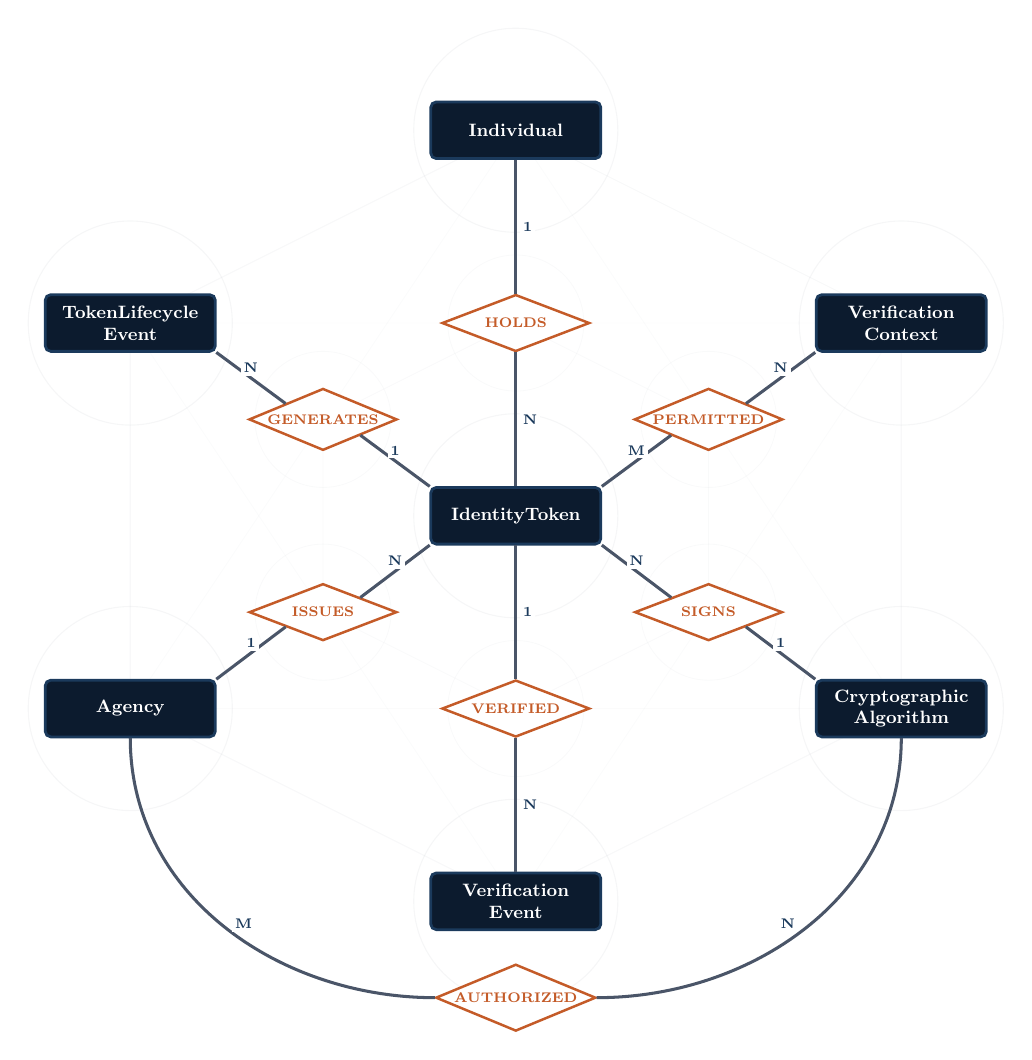
\begin{tikzpicture}[
  scale=0.72, every node/.append style={transform shape},
  font=\small,
  entbox/.style={
    draw=navymid, line width=1pt, rounded corners=2pt,
    minimum width=3.0cm, minimum height=1cm,
    fill=navydark, text=white, font=\bfseries\small,
    align=center,
  },
  reldiamond/.style={
    draw=accent, line width=0.9pt,
    diamond, aspect=2.4,
    minimum width=2.6cm, minimum height=1cm,
    fill=white, text=accent, font=\scriptsize\bfseries,
    align=center, inner sep=1pt,
  },
  link/.style={draw=steelgray, line width=1.1pt},
  card/.style={font=\scriptsize\bfseries\color{navymid},
    fill=white, inner sep=1.5pt},
]

% ====================================================================
% ER DIAGRAM - Metatron's Cube layout, symmetric hexagonal arrangement.
% Primary diagram shows 7 core entities + IdentityToken at center.
% BlockchainAnchor, DeviceBinding, and RevocationList are documented in
% Figure 2 to preserve the symmetric layout.
% ====================================================================

% === BACKGROUND GEOMETRY (Metatron's Cube, subtle) ===
\begin{scope}[on background layer]
  \foreach \pos in {(0,0), (0,6.8), (-6.8,3.4), (6.8,3.4), (-6.8,-3.4), (6.8,-3.4), (0,-6.8)} {
    \draw[steelgray, line width=0.4pt, opacity=0.05] \pos circle (1.8);
  }
  \foreach \pos in {(0,3.4), (-3.4,1.7), (3.4,1.7), (-3.4,-1.7), (3.4,-1.7), (0,-3.4)} {
    \draw[steelgray, line width=0.3pt, opacity=0.03] \pos circle (1.2);
  }
  \draw[steelgray, line width=0.4pt, opacity=0.04]
    (0,6.8) -- (-6.8,3.4) -- (-6.8,-3.4) -- (0,-6.8) -- (6.8,-3.4) -- (6.8,3.4) -- cycle;
  \draw[steelgray, line width=0.3pt, opacity=0.03]
    (0,3.4) -- (-3.4,1.7) -- (-3.4,-1.7) -- (0,-3.4) -- (3.4,-1.7) -- (3.4,1.7) -- cycle;
  \draw[steelgray, line width=0.3pt, opacity=0.025]
    (0,6.8) -- (-6.8,-3.4) -- (6.8,-3.4) -- cycle;
  \draw[steelgray, line width=0.3pt, opacity=0.025]
    (0,-6.8) -- (-6.8,3.4) -- (6.8,3.4) -- cycle;
\end{scope}

% === CENTER ===
\node[entbox] (tok) at (0, 0) {IdentityToken};

% === UPPER TRIANGLE ===
\node[entbox] (ind) at (0, 6.8)       {Individual};
\node[entbox] (tle) at (-6.8, 3.4)    {TokenLifecycle\\Event};
\node[entbox] (ctx) at (6.8, 3.4)     {Verification\\Context};

% === LOWER TRIANGLE ===
\node[entbox] (agy) at (-6.8, -3.4)   {Agency};
\node[entbox] (alg) at (6.8, -3.4)    {Cryptographic\\Algorithm};
\node[entbox] (ve)  at (0, -6.8)      {Verification\\Event};

% --- HOLDS (Individual to Token, vertical) ---
\node[reldiamond] (rel_holds) at (0, 3.4) {HOLDS};
\draw[link] (ind.south) -- (rel_holds.north);
\draw[link] (rel_holds.south) -- (tok.north);
\node[card, right=2pt] at ($(ind.south)!0.5!(rel_holds.north)$) {1};
\node[card, right=2pt] at ($(rel_holds.south)!0.5!(tok.north)$) {N};

% --- GENERATES (Token to TLE) ---
\node[reldiamond] (rel_gen) at (-3.4, 1.7) {GENERATES};
\draw[link] (tok.north west) -- (rel_gen.south east);
\draw[link] (rel_gen.north west) -- (tle.south east);
\node[card, above=1pt] at ($(tok.north west)!0.5!(rel_gen.south east)$) {1};
\node[card, above=1pt] at ($(rel_gen.north west)!0.5!(tle.south east)$) {N};

% --- PERMITTED (Token to VerificationContext, M:N) ---
\node[reldiamond] (rel_perm) at (3.4, 1.7) {PERMITTED};
\draw[link] (tok.north east) -- (rel_perm.south west);
\draw[link] (rel_perm.north east) -- (ctx.south west);
\node[card, above=1pt] at ($(tok.north east)!0.5!(rel_perm.south west)$) {M};
\node[card, above=1pt] at ($(rel_perm.north east)!0.5!(ctx.south west)$) {N};

% --- ISSUES (Agency to Token) ---
\node[reldiamond] (rel_iss) at (-3.4, -1.7) {ISSUES};
\draw[link] (agy.north east) -- (rel_iss.south west);
\draw[link] (rel_iss.north east) -- (tok.south west);
\node[card, above=1pt] at ($(agy.north east)!0.5!(rel_iss.south west)$) {1};
\node[card, above=1pt] at ($(rel_iss.north east)!0.5!(tok.south west)$) {N};

% --- SIGNS (CryptoAlgorithm to Token) ---
\node[reldiamond] (rel_signs) at (3.4, -1.7) {SIGNS};
\draw[link] (alg.north west) -- (rel_signs.south east);
\draw[link] (rel_signs.north west) -- (tok.south east);
\node[card, above=1pt] at ($(alg.north west)!0.5!(rel_signs.south east)$) {1};
\node[card, above=1pt] at ($(rel_signs.north west)!0.5!(tok.south east)$) {N};

% --- VERIFIED (Token to VE, vertical) ---
\node[reldiamond] (rel_ver) at (0, -3.4) {VERIFIED};
\draw[link] (tok.south) -- (rel_ver.north);
\draw[link] (rel_ver.south) -- (ve.north);
\node[card, right=2pt] at ($(tok.south)!0.5!(rel_ver.north)$) {1};
\node[card, right=2pt] at ($(rel_ver.south)!0.5!(ve.north)$) {N};

% --- AUTHORIZED (Agency to CryptoAlgorithm, symmetric arc below VE) ---
\node[reldiamond] (rel_auth) at (0, -8.5) {AUTHORIZED};
\draw[link] (agy.south) to[out=-90, in=180] (rel_auth.west);
\draw[link] (rel_auth.east) to[out=0, in=-90] (alg.south);
\node[card] at (-4.8, -7.2) {M};
\node[card] at (4.8, -7.2) {N};

\end{tikzpicture}

\caption{Core entity--relationship diagram in Chen notation. Navy rectangles are entities; orange diamonds are relationships. Cardinality labels (1, N, M) appear on the connecting lines. The seven core entities are arranged symmetrically around \entity{IdentityToken} at the center. The \entity{Individual} to \entity{IdentityToken} relationship is one-to-many with a partial uniqueness constraint (multiple provisioned tokens, one active at a time). The two M:N relationships (\textsc{Authorized} and \textsc{Permitted}) resolve to junction tables in the relational model. Three additional subsidiary entities (BlockchainAnchor, RevocationList, DeviceBinding) attach directly to \entity{IdentityToken} and are shown separately in Figure~\ref{fig:er-subsidiary}.}
\label{fig:er-core}
\end{figure}

% \newpage  -- removed; let section flow naturally

\textbf{Reading the diagram.} The diagram encodes three design choices through visual structure. \textit{First}, \entity{IdentityToken} sits at the geometric center because every other entity relates to it through exactly one relationship, making the schema a hub-and-spoke topology rather than a peer mesh. \textit{Second}, the four principals (\entity{Individual}, \entity{Agency}, \entity{CryptographicAlgorithm}, \entity{VerificationContext}) are arranged at the four cardinal positions because they are the schema's external authorities --- entities that exist independently of any token and govern what tokens can do. \textit{Third}, the two record-type entities (\entity{TokenLifecycleEvent}, \entity{VerificationEvent}) are placed at the secondary positions because they are existentially dependent on \entity{IdentityToken} and are the high-volume tables in any real deployment. The single peer-to-peer relationship \textsc{Authorized} is rendered as the bottom arc connecting \entity{Agency} and \entity{CryptographicAlgorithm}, distinguishing it from the spokes. This layout is not aesthetic: it makes the schema's information-flow direction immediately legible. Reads flow inward (verifiers consult permissions, contexts, algorithms); writes flow outward (issuance creates token, lifecycle event, and permissions in one transaction); cross-cutting administrative queries (UC-6 algorithm migration, UC-7 warrant audit) traverse the whole topology.

\noindent\textit{Figure~\ref{fig:er-subsidiary} below shows three additional subsidiary entities that attach directly to \entity{IdentityToken}. They are rendered separately from Figure~\ref{fig:er-core} because they are structurally peripheral to the core seven-entity model: each exists only to store data derived from or referencing a specific \entity{IdentityToken}. Placing them on the primary diagram would obscure the symmetric hub-and-spoke relationships among the core entities without adding clarity about their own role.}

\begin{figure}[H]
\centering
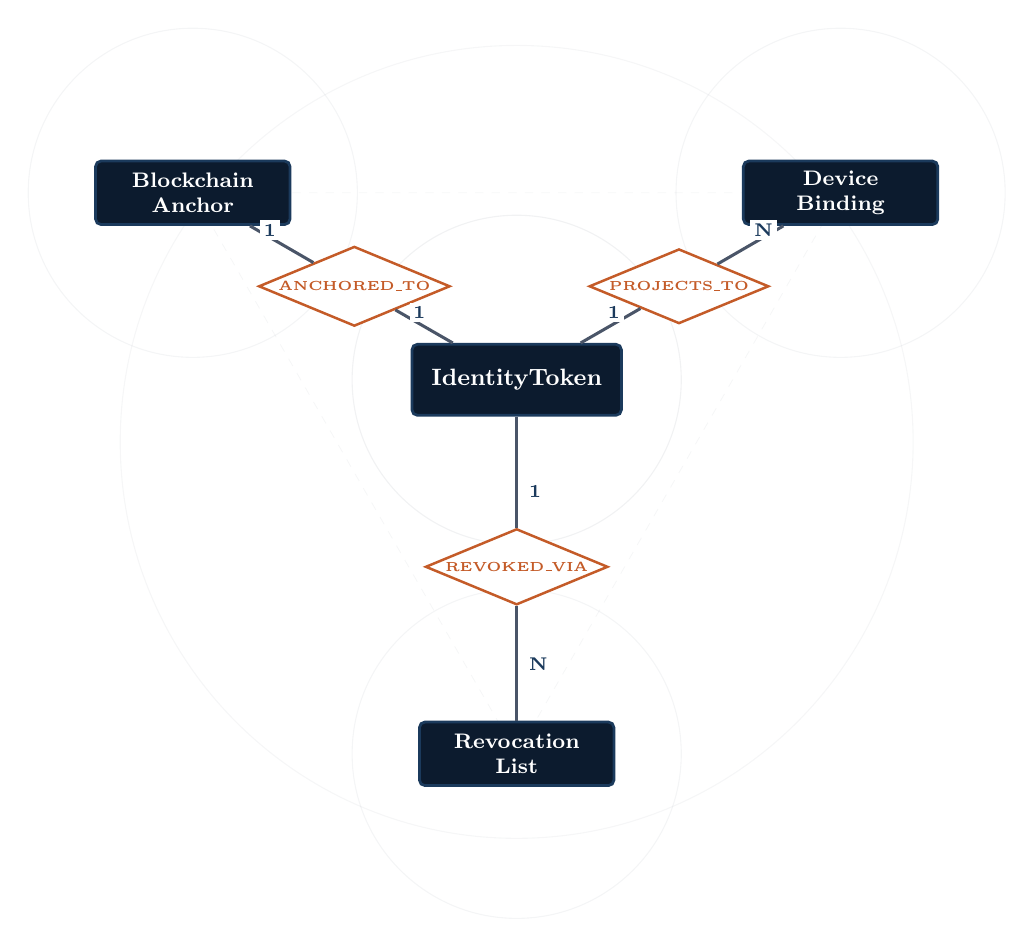
\begin{tikzpicture}[
  scale=0.95, every node/.append style={transform shape},
  font=\small,
  entbox/.style={
    draw=navymid, line width=1pt, rounded corners=2pt,
    minimum width=2.8cm, minimum height=0.95cm,
    fill=navydark, text=white, font=\bfseries\small,
    align=center,
  },
  subbox/.style={
    draw=navymid, line width=1pt, rounded corners=2pt,
    minimum width=2.6cm, minimum height=0.85cm,
    fill=navydark, text=white, font=\bfseries\footnotesize,
    align=center,
  },
  reldiamond/.style={
    draw=accent, line width=0.9pt,
    diamond, aspect=2.4,
    minimum width=2.4cm, minimum height=0.9cm,
    fill=white, text=accent, font=\tiny\bfseries,
    align=center, inner sep=1pt,
  },
  link/.style={draw=steelgray, line width=1.1pt},
  card/.style={font=\scriptsize\bfseries\color{navymid},
    fill=white, inner sep=1.5pt},
]

% === BACKGROUND SACRED GEOMETRY ===
\begin{scope}[on background layer]
  \draw[steelgray, line width=0.4pt, opacity=0.08] (0,0) circle (2.2);
  \draw[steelgray, line width=0.4pt, opacity=0.06] (-4.33, 2.5) circle (2.2);
  \draw[steelgray, line width=0.4pt, opacity=0.06] (4.33, 2.5)  circle (2.2);
  \draw[steelgray, line width=0.4pt, opacity=0.06] (0, -5) circle (2.2);
  \draw[steelgray, line width=0.4pt, opacity=0.05] (0,-0.83) circle (5.3);
  \draw[steelgray, line width=0.3pt, opacity=0.05, dashed]
    (-4.33, 2.5) -- (4.33, 2.5) -- (0, -5) -- cycle;
\end{scope}

% === CENTER: IdentityToken ===
\node[entbox] (tok) at (0, 0) {IdentityToken};

% === THREE SUBSIDIARIES AT 120-DEGREE INTERVALS (r = 5) ===
\node[subbox] (blk) at (-4.33, 2.5) {Blockchain\\Anchor};
\node[subbox] (dev) at (4.33, 2.5)  {Device\\Binding};
\node[subbox] (rev) at (0, -5) {Revocation\\List};

% === RELATIONSHIP DIAMONDS ON SPOKES (r = 2.5) ===
\node[reldiamond] (rel_anch) at (-2.17, 1.25) {ANCHORED\_TO};
\node[reldiamond] (rel_proj) at (2.17, 1.25)  {PROJECTS\_TO};
\node[reldiamond] (rel_rev)  at (0, -2.5)     {REVOKED\_VIA};

% === CONNECTING LINES ===
\draw[link] (tok) -- (rel_anch);
\draw[link] (rel_anch) -- (blk);
\node[card] at (-1.3, 0.9) {1};
\node[card] at (-3.3, 2.0) {1};

\draw[link] (tok) -- (rel_proj);
\draw[link] (rel_proj) -- (dev);
\node[card] at (1.3, 0.9) {1};
\node[card] at (3.3, 2.0) {N};

\draw[link] (tok) -- (rel_rev);
\draw[link] (rel_rev) -- (rev);
\node[card, right=3pt] at (0, -1.5) {1};
\node[card, right=3pt] at (0, -3.8) {N};

\end{tikzpicture}

\caption{\entity{IdentityToken} and its three subsidiary entities, arranged with triadic rotational symmetry around the central token. \entity{BlockchainAnchor} represents optional decentralized-identifier anchoring on a post-quantum-capable distributed ledger (discussed as an alternative trust architecture in the Limitations section). \entity{RevocationList} is a verifier-facing historical revocation registry, separating revocation publication from the token's own status field so that verifiers can perform audit-accurate freshness checks. \entity{DeviceBinding} represents on-device digital projections of the physical token stored in a device's secure enclave (no cloud storage). All three attach to \entity{IdentityToken} but are shown separately from the core diagram for clarity.}
\label{fig:er-subsidiary}
\end{figure}

The split between Figures~\ref{fig:er-core} and~\ref{fig:er-subsidiary} reflects a design distinction, not a layout convenience. The seven core entities are \textit{constitutive}: each represents a principal that the system is fundamentally about (people, authorities, algorithms, contexts, the credential itself, and the two records the credential generates over its lifetime). Removing any of them collapses the model. The three subsidiary entities are \textit{derivative}: each exists to serve a specific operational requirement that does not arise in the conceptual model itself but does arise once the schema is deployed against real verifiers. \entity{DeviceBinding} exists because verifiers accept digital presentation; \entity{BlockchainAnchor} exists because some trust models prefer ledger-anchored identifiers; \entity{RevocationList} exists because verifier-side freshness checks need a publication channel distinct from the token's own status field. They attach to \entity{IdentityToken} as derivative records rather than as participants in the symmetric hub-and-spoke topology of the core diagram. The two diagrams together specify the complete schema; their separation makes the architectural distinction legible.

% \newpage  -- removed; let section flow naturally
\needspace{3\baselineskip}
\subsection{Entity Reference}

The ER diagrams above show entity names and relationships only. Complete attribute specifications appear in Table~\ref{tab:entities}. Primary keys are shown in \textbf{\underline{bold underlined}} text; foreign keys are shown in \textit{\underline{italic underlined}} text.

The attribute set for each entity is the minimum needed to answer the operational queries from §\ref{sec:info-collection} and the constraint requirements from §\ref{sec:db-requirements}. Three conventions apply throughout: primary keys are surrogate \texttt{SERIAL} integers (natural keys would propagate mutability and sensitivity through the FK structure); enumerated fields appear in italic with their fixed domain listed parenthetically (these are enforced by \texttt{CHECK} constraints at the schema level); and sensitive data the system refuses to store --- raw biometric templates, plaintext genomic sequences, token-identifying data on \texttt{ZERO\_KNOWLEDGE} verifications --- is conspicuously absent from the attribute lists. The schema's privacy posture is visible in what it refuses to record, not only in what it constrains.

\begin{table}[H]
\centering
\footnotesize
\caption{Complete attribute reference for all entities.}
\label{tab:entities}
\setlength{\tabcolsep}{5pt}
\renewcommand{\arraystretch}{1.15}
\rowcolors{2}{tabstripe}{white}
\begin{tabularx}{\textwidth}{>{\bfseries}p{1.62in} >{\RaggedRight\arraybackslash}X}
\toprule
\rowcolor{tabheader}
\thead{Entity} & \thead{Attributes} \\
\midrule
Individual & \pk{individual\_id}, \texttt{legal\_name}, \texttt{date\_of\_birth}, \texttt{jurisdiction}, \texttt{enrollment\_date} \\
Agency & \pk{agency\_id}, \texttt{name}, \texttt{agency\_type}, \texttt{jurisdiction}, \texttt{authorization\_level} \\
CryptographicAlgorithm & \pk{algorithm\_id}, \texttt{name}, \texttt{family}, \texttt{quantum\_resistant}, \texttt{nist\_standard}, \texttt{security\_level\_bits}, \texttt{public\_key\_size}, \texttt{signature\_size}, \texttt{deprecation\_date} \\
VerificationContext & \pk{context\_id}, \texttt{context\_type} \textit{(BANKING, EMPLOYMENT, HEALTHCARE, TRAVEL, VOTING, MOTOR\_VEHICLE, GOVERNMENT\_BENEFITS)}, \texttt{description}, \texttt{requires\_biometric}, \texttt{min\_security\_level} \\
IdentityToken & \pk{token\_id}, \texttt{token\_value}, \texttt{physical\_serial}, \texttt{hardware\_model}, \texttt{biometric\_binding\_type} \textit{(NONE, FINGERPRINT, FACE, IRIS)}, \texttt{biometric\_enrolled\_date}, \fk{enrollment\_witness\_agency\_id}, \texttt{liveness\_check\_type} \textit{(PASSIVE, ACTIVE\_CHALLENGE, MULTI\_MODAL)}, \fk{individual\_id}, \fk{issuing\_agency\_id}, \fk{algorithm\_id}, \fk{predecessor\_token\_id}, \texttt{activation\_sequence}, \texttt{status} \textit{(ACTIVE, RESERVE, DORMANT, REVOKED, LOST, EXPIRED)}, \texttt{issued\_date}, \texttt{activated\_date}, \texttt{expiration\_date} \\
TokenLifecycleEvent & \pk{event\_id}, \fk{token\_id}, \fk{actor\_agency\_id}, \texttt{event\_type} \textit{(ISSUED, ACTIVATED, DEACTIVATED, DEVICE\_BOUND, DEVICE\_REVOKED, REVOKED, LOST, EXPIRED, REPLACED)}, \texttt{event\_timestamp}, \texttt{reason\_code} \\
VerificationEvent & \pk{event\_id}, \fk{token\_id} \textit{(nullable)}, \fk{requesting\_agency\_id}, \fk{context\_id}, \texttt{event\_timestamp}, \texttt{outcome} \textit{(SUCCESS, FAILURE, EXPIRED, UNAUTHORIZED)}, \texttt{disclosure\_level} \textit{(ZERO\_KNOWLEDGE, SELECTIVE, FULL)}, \texttt{proof\_commitment}, \texttt{requestor\_location} \\
DeviceBinding & \pk{binding\_id}, \fk{token\_id}, \texttt{device\_type} \textit{(PHONE, TABLET, WATCH)}, \texttt{device\_fingerprint}, \texttt{binding\_method}, \texttt{authorized\_date}, \texttt{expires\_date}, \texttt{status} \textit{(ACTIVE, REVOKED)}, \texttt{revocation\_reason} \\
BlockchainAnchor & \pk{anchor\_id}, \fk{token\_id}, \texttt{did}, \texttt{commitment\_hash}, \texttt{ledger\_network} \textit{(ALGORAND\_PQ, HYPERLEDGER\_INDY, CUSTOM\_LATTICE)}, \texttt{anchor\_tx\_hash}, \texttt{anchored\_date}, \texttt{status} \textit{(ACTIVE, SUPERSEDED, REVOKED)} \\
RevocationList & \pk{revocation\_id}, \fk{token\_id}, \fk{revoked\_by\_agency\_id}, \texttt{revocation\_timestamp}, \texttt{effective\_date}, \texttt{reason\_code} \textit{(COMPROMISED, LOST, STOLEN, SUPERSEDED, ADMINISTRATIVE, DEATH)}, \texttt{published\_location} \\
\midrule
\rowcolor{tabstripe}
\textit{AgencyAlgorithmAuth} & \pk{agency\_id}, \pk{algorithm\_id}, \texttt{authorization\_type}, \texttt{authorized\_date} \textit{(M:N junction for \textsc{Authorized})} \\
\textit{TokenPermission} & \pk{token\_id}, \pk{context\_id}, \texttt{permission\_level}, \texttt{granted\_date} \textit{(M:N junction for \textsc{Permitted})} \\
\bottomrule
\end{tabularx}
\end{table}

\textit{Note:} The two junction tables at the bottom of the table do not appear on the ER diagram because they represent the implementation-level resolution of the M:N relationships \textsc{Authorized} and \textsc{Permitted}. They appear as explicit relations in the relational model and as \texttt{CREATE TABLE} statements in the SQL implementation. The \texttt{status} column on \entity{IdentityToken} admits the six values shown above (\texttt{ACTIVE}, \texttt{RESERVE}, \texttt{DORMANT}, \texttt{REVOKED}, \texttt{LOST}, \texttt{EXPIRED}); the legal transitions among them are formalized in Appendix~\ref{app:state-machine}. Tokens are never deleted from the schema. When a token's lifecycle ends, the record is retained in a terminal status for audit purposes, and a new token is issued as a full replacement.

\subsection{Relationship Catalog}

\begin{table}[H]
\centering
\footnotesize
\caption{Relationships, cardinalities, and design notes.}
\label{tab:relationships}
\setlength{\tabcolsep}{4pt}
\renewcommand{\arraystretch}{1.1}
\rowcolors{2}{tabstripe}{white}
\begin{tabularx}{\textwidth}{>{\RaggedRight\arraybackslash}p{1.95in} >{\centering\arraybackslash}p{0.85in} >{\RaggedRight\arraybackslash}X}
\toprule
\rowcolor{tabheader}
\thead{Relationship} & \thead{Cardinality} & \thead{Notes} \\
\midrule
Individual \textsc{Holds} IdentityToken & 1:N & One person, one active credential, plus optional reserves. Enforced by a partial \texttt{UNIQUE} index on \texttt{individual\_id} where \texttt{status = 'ACTIVE'}. \\
Agency \textsc{Issues} IdentityToken & 1:N & An issuing agency creates many tokens. Each token has exactly one issuer. \\
CryptographicAlgorithm \textsc{Signs} IdentityToken & 1:N & One algorithm signs many tokens. Deprecated algorithms define a queryable replacement cohort. \\
IdentityToken \textsc{Projects\_To} DeviceBinding & 1:N & A token may authorize a small number of personal device bindings (typically $\leq 3$). Each binding stores a cryptographic copy in the device's secure enclave; nothing is stored in the cloud. \\
IdentityToken \textsc{Anchored\_To} BlockchainAnchor & 0..1:1 & An optional decentralized-identifier anchor on a post-quantum-capable distributed ledger. The relationship is mandatory on the \entity{BlockchainAnchor} side (every anchor references exactly one token) and optional on the \entity{IdentityToken} side (a token may have zero or one anchor). Holds commitments and references only, never personal or biometric data. Supports the alternative trust architecture noted in Limitations. \\
IdentityToken \textsc{Revoked\_Via} RevocationList & 1:N & A token may have zero, one, or multiple revocation records. Separating revocation from the token's own status field allows audit-accurate historical freshness checks by verifiers. \\
IdentityToken $\rightarrow$ IdentityToken (predecessor) & 0:1 & Self-referential FK capturing which token this token succeeded when a reserve was activated. Null for the first token in a holder's sequence. \\
Agency \textsc{Authorized} CryptographicAlgorithm & M:N & Resolved via \entity{AgencyAlgorithmAuth}. Authorization is type-scoped (ISSUE, VERIFY, BOTH). \\
IdentityToken \textsc{Permitted} VerificationContext & M:N & Resolved via \entity{TokenPermission}. A token may be authorized for multiple contexts at different permission levels. \\
IdentityToken \textsc{Generates} TokenLifecycleEvent & 1:N & Append-only audit trail: ISSUED, ACTIVATED, DEACTIVATED, DEVICE\_BOUND, DEVICE\_REVOKED, REVOKED, LOST, EXPIRED, REPLACED. \\
IdentityToken \textsc{Verified} VerificationEvent & 1:N & High-volume relationship. A token generates thousands of verification events over its operational life. \\
\midrule
\textit{VerificationContext} $\rightarrow$ VerificationEvent & 1:N & Captured as FK (\texttt{context\_id}). Each verification occurs in exactly one context, which determines the minimum security level required. \\
\textit{Agency} $\rightarrow$ VerificationEvent & 1:N & Captured as FK (\texttt{requesting\_agency\_id}). Agency plays both issuer and verifier roles, distinguished by which FK column references it. \\
\bottomrule
\end{tabularx}
\end{table}

\subsection{Design Notes}

\textbf{One active credential per person, multiple provisioned.} Each individual may have several tokens provisioned and bound to them, but only one may be in \texttt{ACTIVE} state at a time, enforced by a partial unique index on \texttt{individual\_id} where \texttt{status='ACTIVE'}. Reserve tokens sit in \texttt{RESERVE} state, pre-issued against the possibility of loss or compromise of the active token; activating a reserve transitions it to \texttt{ACTIVE} and transitions the former active token to \texttt{DORMANT}. The full sequence is preserved through \texttt{activation\_sequence} and a self-referential \texttt{predecessor\_token\_id} foreign key. \textbf{Device projection without cloud storage.} \entity{DeviceBinding} represents phone, tablet, or watch copies of the physical token, each stored in the device's secure enclave; no backup credential is ever stored on a server, and the database records only binding metadata (device fingerprint, authorization window, revocation status). Losing a phone means revoking its binding without affecting the physical token or other device bindings. \textbf{Agency plays dual roles through distinct foreign keys.} An \entity{Agency} row can be referenced as an issuing agency on \entity{IdentityToken} (\texttt{issuing\_agency\_id}) and as a requesting agency on \entity{VerificationEvent} (\texttt{requesting\_agency\_id}); the two roles are disambiguated by which FK column holds the reference, and the \entity{AgencyAlgorithmAuth} junction further constrains which agencies may issue, verify, or both, per algorithm.

\textbf{Quantum-resistance is a first-class attribute.} \entity{CryptographicAlgorithm} stores a \texttt{quantum\_resistant} boolean alongside algorithm family, NIST standard designation, and security level in bits, enabling direct SQL queries for tokens at risk from harvest-now-decrypt-later attacks. \textbf{VerificationContext is a separate entity rather than an enum.} Contexts carry per-context metadata (\texttt{requires\_biometric}, \texttt{min\_security\_level}) and participate in the M:N \entity{TokenPermission} relationship; modeling context as a string column would forfeit both capabilities. \textbf{Junction tables live in the relational model, not the ER diagram.} The two M:N relationships (\textsc{Authorized}, \textsc{Permitted}) are shown as single diamond relationships on the ER diagram following Chen-notation convention; their resolution into \entity{AgencyAlgorithmAuth} and \entity{TokenPermission} occurs when the ER model is mapped to relations.

\textbf{Disclosure level is a column on the verification record, not a query parameter.} The decision to store \texttt{disclosure\_level} as a persisted attribute of \entity{VerificationEvent} (rather than as runtime configuration on the verifier) is the architectural choice that distinguishes this design from comparable systems (Appendix~\ref{app:comparison}). Verifiers cannot retroactively elevate a \texttt{ZERO\_KNOWLEDGE} record to \texttt{FULL} disclosure: the database literally never stored the identifying fields. The \texttt{chk\_disclosure\_token\_consistency} check enforces this at insert time, requiring \texttt{token\_id IS NULL} for \texttt{ZERO\_KNOWLEDGE} events and \texttt{token\_id IS NOT NULL} for \texttt{FULL} events. \textbf{Lifecycle and verification events are append-only by tooling.} NFR-4 requires every state change to be auditable; \entity{TokenLifecycleEvent} and \entity{VerificationEvent} are append-only at the trigger layer (the reference implementation blocks \texttt{UPDATE} and \texttt{DELETE} on both), with administrative deletion requiring explicit trigger removal --- a deliberate friction point that produces an auditable record of any override.


% ============================================================================
% STEP 5: RELATIONAL MODEL
% ============================================================================
% \newpage  -- removed; let section flow naturally
\section{Relational Model}
\label{sec:rel-model}

\subsection{Entity-to-Table Mapping}

Each of the ten entities maps directly to a table. The two many-to-many relationships are resolved via junction tables with composite primary keys, producing twelve tables in total.

\begin{table}[H]
\centering
\footnotesize
\caption{Entity-to-table mapping.}
\rowcolors{2}{tabstripe}{white}
\begin{tabularx}{\textwidth}{l l >{\RaggedRight\arraybackslash}X}
\toprule
\rowcolor{tabheader}
\thead{ER Entity} & \thead{Relational Table} & \thead{Notes} \\
\midrule
\entity{Individual} & \texttt{Individual} & Core person record \\
\entity{Agency} & \texttt{Agency} & Dual role (issuer + verifier) \\
\entity{CryptographicAlgorithm} & \texttt{CryptographicAlgorithm} & Post-quantum + classical support \\
\entity{VerificationContext} & \texttt{VerificationContext} & 7 fixed contexts with metadata \\
\entity{IdentityToken} & \texttt{IdentityToken} & \textbf{Central hub} with multiple FKs \\
\entity{TokenLifecycleEvent} & \texttt{TokenLifecycleEvent} & Append-only audit trail \\
\entity{VerificationEvent} & \texttt{VerificationEvent} & High-volume transactional table \\
\entity{DeviceBinding} & \texttt{DeviceBinding} & 1:N subsidiary \\
\entity{BlockchainAnchor} & \texttt{BlockchainAnchor} & Optional DID anchoring (1:1) \\
\entity{RevocationList} & \texttt{RevocationList} & Historical revocation records \\
\midrule
\entity{AgencyAlgorithmAuth} & \texttt{AgencyAlgorithmAuth} & Junction (M:N \textsc{Authorized}) \\
\entity{TokenPermission} & \texttt{TokenPermission} & Junction (M:N \textsc{Permitted}) \\
\bottomrule
\end{tabularx}
\end{table}

\subsection{Relationship Mapping}

\textbf{One-to-Many (1:N).} Each 1:N relationship is implemented by placing a foreign key on the table corresponding to the \textit{many} side. \entity{IdentityToken} therefore carries \texttt{individual\_id} (from \textsc{Holds}), \texttt{issuing\_agency\_id} (from \textsc{Issues}), \texttt{algorithm\_id} (from \textsc{Signs}), and \texttt{enrollment\_witness\_agency\_id} (a secondary reference into \entity{Agency}). \entity{TokenLifecycleEvent}, \entity{VerificationEvent}, \entity{DeviceBinding}, \entity{BlockchainAnchor}, and \entity{RevocationList} each carry \texttt{token\_id}. \entity{VerificationEvent} additionally carries \texttt{requesting\_agency\_id} and \texttt{context\_id}; \entity{TokenLifecycleEvent} carries \texttt{actor\_agency\_id}; \entity{RevocationList} carries \texttt{revoked\_by\_agency\_id}. The \texttt{token\_id} on \entity{VerificationEvent} is nullable so that \texttt{ZERO\_KNOWLEDGE} verifications produce no token-identifying record.

\textbf{Many-to-Many (M:N).} Each M:N relationship resolves to a junction table with a composite primary key on the two FK columns, plus relationship-specific attributes. \entity{AgencyAlgorithmAuth} has primary key \texttt{(agency\_id, algorithm\_id)} and carries \texttt{authorization\_type} (\texttt{ISSUE}, \texttt{VERIFY}, or \texttt{BOTH}). \entity{TokenPermission} has primary key \texttt{(token\_id, context\_id)} and carries \texttt{permission\_level} (\texttt{READ}, \texttt{VERIFY}, or \texttt{FULL}).

\textbf{Self-referential (0:1).} \texttt{IdentityToken.predecessor\_token\_id} references \texttt{IdentityToken.token\_id} on the same table. The reference is nullable; the first token in any holder's sequence has no predecessor.

\textbf{One-to-one (1:1).} \entity{BlockchainAnchor} carries \texttt{token\_id} as a foreign key with the application-level invariant that at most one anchor exists per token in \texttt{ACTIVE} status (additional anchors are permitted in \texttt{SUPERSEDED} or \texttt{REVOKED} status).

\subsection{Schema-Level Constraints Summary}

Four schema-level constraints carry architectural weight. \textbf{Partial uniqueness} on \texttt{individual\_id} where \texttt{status='ACTIVE'} is implemented as a partial \texttt{UNIQUE} index, restricting each individual to one active token at a time while permitting any number of \texttt{RESERVE}, \texttt{DORMANT}, and terminal-state tokens. \textbf{\texttt{CHECK} constraints} on every enumerated field guarantee that no invalid status, type, or context value can be inserted (\texttt{status} on \entity{IdentityToken}, \texttt{outcome} and \texttt{disclosure\_level} on \entity{VerificationEvent}, \texttt{event\_type} on \entity{TokenLifecycleEvent}, etc.). \textbf{Foreign-key integrity} is enforced on every cross-entity reference; cascades are explicitly avoided so that audit records persist even if their parent token is removed (in practice, tokens are never removed, only transitioned through \texttt{REVOKED}, \texttt{LOST}, or \texttt{EXPIRED}). \textbf{Indexes} on high-query columns (\texttt{individual\_id}, \texttt{status}, \texttt{event\_timestamp}, \texttt{context\_id}, \texttt{token\_id} on lifecycle and verification tables) support the verification and audit query patterns.

\subsection{Mapping Rules Applied}

The relational model above derives from five standard ER-to-relational mapping rules (Elmasri \& Navathe, ch. 9), each applied without modification. \textbf{Rule 1 (strong-entity mapping):} each of the ten ER entities maps to a table with the entity's primary key as table primary key. \textbf{Rule 2 (weak-entity mapping):} no weak entities exist in this schema; all record-type entities (\entity{TokenLifecycleEvent}, \entity{VerificationEvent}, \entity{DeviceBinding}, \entity{BlockchainAnchor}, \entity{RevocationList}) carry their own surrogate primary key. \textbf{Rule 3 (1:1 relationships):} the single 0..1:1 (\entity{IdentityToken} \textsc{Anchored\_To} \entity{BlockchainAnchor}) places the FK on the optional side. \textbf{Rule 4 (1:N relationships):} FK on the \textit{many} side, applied seven times across \entity{IdentityToken}, \entity{TokenLifecycleEvent}, \entity{VerificationEvent}, \entity{DeviceBinding}, and \entity{RevocationList}. \textbf{Rule 5 (M:N relationships):} junction table with composite primary key, applied twice (\entity{AgencyAlgorithmAuth} resolving \textsc{Authorized}; \entity{TokenPermission} resolving \textsc{Permitted}), each carrying relationship-specific attributes (\texttt{authorization\_type} and \texttt{permission\_level}). The self-referential FK on \entity{IdentityToken} (\texttt{predecessor\_token\_id}) is a direct application of Rule 4 with the same table on both sides. The result is twelve tables, eighteen foreign keys (including the self-referential \texttt{predecessor\_token\_id}), fourteen \texttt{CHECK} constraints, and one partial unique index. The full inventory is enumerated in the SQL implementation that follows.

\subsection{Normalization Analysis}
\label{subsec:normalization}

The mapping rules produce a schema; they do not prove the schema is well-formed. This subsection establishes that every relation is in Boyce-Codd Normal Form (BCNF). The proof proceeds by enumerating the functional dependencies (FDs) on each relation and confirming the left-hand side of every nontrivial FD is a superkey.

\textbf{First Normal Form.} Every attribute holds an atomic value drawn from a defined domain. Multi-valued or composite attributes are not used: the seven \texttt{VerificationContext} values are rows in a separate entity rather than a comma-separated string; multiple device bindings per token are rows in \entity{DeviceBinding}; M:N relationships are resolved through junction tables. 1NF holds by construction.

\textbf{Functional dependencies.} The nontrivial FDs fall into two patterns. On every entity table, the surrogate primary key determines all other attributes (\texttt{token\_id} $\to$ all other columns of \entity{IdentityToken}; \texttt{individual\_id} $\to$ all other columns of \entity{Individual}; and so on). No other nontrivial FDs hold because the primary key is surrogate (a system-generated \texttt{SERIAL}) rather than derived from any application attribute, so no application attribute determines any other on the same row. On the two junction tables, the composite key determines the relationship-specific attributes: \texttt{(agency\_id, algorithm\_id)} $\to$ \texttt{(authorization\_type, authorized\_date)} on \entity{AgencyAlgorithmAuth}, and \texttt{(token\_id, context\_id)} $\to$ \texttt{(permission\_level, granted\_date)} on \entity{TokenPermission}.

\textbf{2NF, 3NF, and BCNF.} 2NF requires that no non-key attribute depend on a proper subset of a composite key. On both junction tables the non-key attributes are properties of the relationship rather than of either key column alone, so no partial dependency exists. 3NF additionally requires no transitive dependency: every non-key attribute is determined directly by the primary key, so 3NF holds. BCNF strengthens 3NF by requiring that the left-hand side of every nontrivial FD be a superkey; since the only nontrivial FDs are those listed above, and each left-hand side is the primary key (a superkey by definition), BCNF holds on every relation. The schema is in BCNF without further decomposition. The \texttt{UNIQUE (individual\_id, status) WHERE status='ACTIVE'} constraint does not affect this analysis: it is a \textit{conditional} uniqueness implementing an application invariant as a partial index, not a relational dependency in the formal sense.

\textbf{Apparent denormalization, addressed.} Two columns warrant explicit comment. \entity{TokenLifecycleEvent}.\texttt{actor\_agency\_id} appears redundant against \entity{IdentityToken}.\texttt{issuing\_agency\_id} but is not: the actor on a lifecycle event is the agency that performed the specific transition, frequently \textit{not} the issuing agency (a revocation may be performed by a different jurisdiction; a device-binding event has no agency actor and the column is nullable). The two columns capture different facts, no FD holds between them, and the relation remains in BCNF. \entity{VerificationEvent}.\texttt{requesting\_agency\_id} and \texttt{context\_id} are similarly independent: one agency verifies across many contexts and one context is exercised by many agencies.

\subsection{Sample DML Operations}

The mapping rules above are necessary but not sufficient: the schema must also be exercisable through transactional DML that preserves every constraint. The two listings below show how the use cases from the requirements analysis translate into SQL, demonstrating that the schema operates correctly under realistic write patterns.

\needspace{3\baselineskip}
\textbf{UC-1 (new token issuance) as a single transaction.} The active-token uniqueness invariant requires the \texttt{INSERT} into \entity{IdentityToken} and the paired \entity{TokenLifecycleEvent} to commit together. The partial unique index on \texttt{individual\_id} where \texttt{status='ACTIVE'} permits this naturally: the new token enters at status \texttt{RESERVE} (outside the index predicate, no uniqueness check) before the activation update transitions it into \texttt{ACTIVE}.

\begin{lstlisting}[language=SQL]
BEGIN;
  INSERT INTO Individual (legal_name, date_of_birth, jurisdiction, enrollment_date)
  VALUES ('A. Holder', '2000-04-15', 'US-PA', CURRENT_TIMESTAMP)
  RETURNING individual_id;
  -- assume returned individual_id = 6

  INSERT INTO IdentityToken (token_value, physical_serial, hardware_model,
                             biometric_binding_type, individual_id,
                             issuing_agency_id, algorithm_id, status,
                             activated_date, expiration_date)
  VALUES ('TKN-PA-2026-000006', 'SN-PA-006', 'TitanQ-3',
          'IRIS', 6, 1, 2, 'ACTIVE',
          CURRENT_TIMESTAMP, CURRENT_DATE + INTERVAL '10 years')
  RETURNING token_id;
  -- assume returned token_id = 6

  INSERT INTO TokenLifecycleEvent (token_id, actor_agency_id, event_type, reason_code)
  VALUES (6, 1, 'ISSUED', 'INITIAL_ENROLLMENT'),
         (6, 1, 'ACTIVATED', 'POST_BIOMETRIC_ENROLLMENT');

  INSERT INTO TokenPermission (token_id, context_id, permission_level)
  VALUES (6, 1, 'VERIFY'),  -- BANKING
         (6, 4, 'VERIFY'),  -- TRAVEL
         (6, 6, 'VERIFY');  -- MOTOR_VEHICLE
COMMIT;
\end{lstlisting}

\needspace{15\baselineskip}
\textbf{UC-4 (reserve activation after loss) requires two status changes on the same individual.} The transitions are ordered: the lost token moves to its terminal status \textit{first} (releasing it from the partial unique index's predicate), then the reserve transitions to \texttt{ACTIVE}. The partial unique index is never violated mid-transaction. This ordering eliminates the need for deferred-constraint semantics:

\begin{lstlisting}[language=SQL]
BEGIN;
  -- Demote the lost token
  UPDATE IdentityToken SET status = 'LOST' WHERE token_id = 3;
  INSERT INTO TokenLifecycleEvent (token_id, actor_agency_id, event_type, reason_code)
  VALUES (3, 1, 'LOST', 'HOLDER_REPORTED_LOSS');
  INSERT INTO RevocationList (token_id, revoked_by_agency_id, reason_code,
                              effective_date, published_location)
  VALUES (3, 1, 'LOST', CURRENT_DATE,
          'https://crl.idtoken.gov/2026/04');

  -- Promote a reserve token to ACTIVE on the same individual
  UPDATE IdentityToken
     SET status = 'ACTIVE',
         predecessor_token_id = 3,
         activation_sequence = 2,
         activated_date = CURRENT_TIMESTAMP
   WHERE individual_id = 2 AND status = 'RESERVE';
  INSERT INTO TokenLifecycleEvent (token_id, actor_agency_id, event_type, reason_code)
  SELECT token_id, 1, 'ACTIVATED', 'RESERVE_PROMOTION'
    FROM IdentityToken
   WHERE individual_id = 2 AND status = 'ACTIVE';
COMMIT;
\end{lstlisting}

Both transactions exercise the schema's distinguishing constraints (the partial uniqueness on \texttt{individual\_id} where \texttt{status='ACTIVE'}, the FK chain across \entity{IdentityToken}, \entity{TokenLifecycleEvent}, and \entity{RevocationList}, and the self-referential \texttt{predecessor\_token\_id} link) and demonstrate that the schema is operationally complete, not merely structurally correct.

% ============================================================================
% STEP 6: SQL IMPLEMENTATION
% ============================================================================
% \newpage  -- removed; let Relational Model flow into SQL Implementation
\section{SQL Implementation}
\label{sec:sql-impl}

The complete SQL script (\texttt{identity\_token\_system.sql}) implements the full schema, populates it with sample data, and defines a utility view. This section presents the schema overview, the most architecturally significant \texttt{CREATE TABLE} statements, and the sample-data summary. The full script is provided alongside this report and runs cleanly on PostgreSQL 14 or later.

\subsection{Schema Overview}

\begin{table}[H]
\centering
\footnotesize
\caption{SQL implementation summary.}
\setlength{\tabcolsep}{5pt}
\renewcommand{\arraystretch}{1.1}
\rowcolors{2}{tabstripe}{white}
\begin{tabularx}{\textwidth}{>{\bfseries}p{1.75in} c >{\RaggedRight\arraybackslash}X}
\toprule
\rowcolor{tabheader}
\thead{Component} & \thead{Count} & \thead{Notes} \\
\midrule
Tables & 12 & 10 entity tables + 2 junction tables \\
Foreign keys & 18 & Including 1 self-referential FK on \entity{IdentityToken} \\
\texttt{CHECK} constraints & 14 & On every enumerated field across all tables \\
Composite primary keys & 2 & On \entity{AgencyAlgorithmAuth} and \entity{TokenPermission} \\
Partial unique constraints & 1 & Deferrable, on \texttt{(individual\_id, status)} \\
Indexes & 5 & On high-query columns supporting verification and audit \\
Views & 1 & \texttt{ActiveTokens} for human-readable active-token summary \\
\midrule
Sample rows & 73 & 5 individuals, 6 agencies, 5 algorithms, 7 contexts, 5 tokens, 9 lifecycle events, 8 verification events, 5 device bindings, 2 blockchain anchors, 1 revocation, 9 authorization grants, 11 permission grants \\
\bottomrule
\end{tabularx}
\end{table}

\needspace{3\baselineskip}
\subsection{Core Table: \texttt{IdentityToken}}

This is the schema's central table. Its \texttt{CREATE TABLE} statement carries six foreign keys (one self-referential), the partial unique index that enforces one active token per individual, and \texttt{CHECK} constraints on three enumerated columns.

\begin{lstlisting}[language=SQL]
CREATE TABLE IdentityToken (
    token_id                     SERIAL PRIMARY KEY,
    token_value                  VARCHAR(128) NOT NULL UNIQUE,
    physical_serial              VARCHAR(64)  NOT NULL UNIQUE,
    hardware_model               VARCHAR(50),
    biometric_binding_type       VARCHAR(20)  NOT NULL
        CHECK (biometric_binding_type IN ('NONE','FINGERPRINT','FACE','IRIS')),
    biometric_enrolled_date      TIMESTAMP,
    enrollment_witness_agency_id INTEGER REFERENCES Agency(agency_id),
    liveness_check_type          VARCHAR(20)
        CHECK (liveness_check_type IN ('PASSIVE','ACTIVE_CHALLENGE','MULTI_MODAL')),
    individual_id                INTEGER NOT NULL REFERENCES Individual(individual_id),
    issuing_agency_id            INTEGER NOT NULL REFERENCES Agency(agency_id),
    algorithm_id                 INTEGER NOT NULL REFERENCES CryptographicAlgorithm(algorithm_id),
    predecessor_token_id         INTEGER REFERENCES IdentityToken(token_id),
    activation_sequence          INTEGER DEFAULT 1,
    status                       VARCHAR(20) NOT NULL DEFAULT 'RESERVE'
        CHECK (status IN ('ACTIVE','RESERVE','DORMANT','REVOKED','LOST','EXPIRED')),
    issued_date                  TIMESTAMP DEFAULT CURRENT_TIMESTAMP,
    activated_date               TIMESTAMP,
    expiration_date              DATE
);

-- One-active-per-person invariant (partial unique index, see Appendix B):
CREATE UNIQUE INDEX uq_one_active_per_person
    ON IdentityToken (individual_id) WHERE status = 'ACTIVE';
\end{lstlisting}

\needspace{3\baselineskip}
\subsection{Junction Table: \texttt{TokenPermission}}

This is the resolution of the M:N \textsc{Permitted} relationship. The composite primary key on \texttt{(token\_id, context\_id)} both enforces the relational integrity of the junction and implements the application-level guarantee that a given (token, context) pair has exactly one permission level at any time.

\begin{lstlisting}[language=SQL]
CREATE TABLE TokenPermission (
    token_id          INTEGER NOT NULL REFERENCES IdentityToken(token_id),
    context_id        INTEGER NOT NULL REFERENCES VerificationContext(context_id),
    permission_level  VARCHAR(20) NOT NULL
        CHECK (permission_level IN ('READ','VERIFY','FULL')),
    granted_date      TIMESTAMP DEFAULT CURRENT_TIMESTAMP,
    PRIMARY KEY (token_id, context_id)
);
\end{lstlisting}

\needspace{3\baselineskip}
\subsection{Utility View: \texttt{ActiveTokens}}

A single view supports the most common operational read pattern: human-readable summaries of every active token with its holder, issuer, and algorithm. The view enables UC-6 (algorithm migration audit) and the operational dashboard described in subsequent project work.

\begin{lstlisting}[language=SQL]
CREATE OR REPLACE VIEW ActiveTokens AS
SELECT  t.token_id,
        i.legal_name,
        a.name   AS issuing_agency,
        alg.name AS algorithm,
        t.status,
        t.activated_date
FROM    IdentityToken t
JOIN    Individual              i  ON t.individual_id     = i.individual_id
JOIN    Agency                  a  ON t.issuing_agency_id = a.agency_id
JOIN    CryptographicAlgorithm  alg ON t.algorithm_id     = alg.algorithm_id
WHERE   t.status = 'ACTIVE';
\end{lstlisting}

\subsection{Sample Data Summary}

The script populates the schema with realistic data representing a microcosm of the system in operation. Five individuals hold five tokens issued by three different federal and state agencies. The \entity{CryptographicAlgorithm} catalog contains five entries (four post-quantum, one deprecated classical retained for migration tracking); the five sample tokens are all signed under post-quantum algorithms, while the classical algorithm appears in \entity{AgencyAlgorithmAuth} only as a historical authorization record. Eight verification events span four contexts (banking, employment, travel, government benefits) at all three disclosure levels. Two tokens carry blockchain anchors (representing the optional DID architecture). One token has been superseded and appears in the revocation list. Eleven \entity{TokenPermission} entries grant context-scoped verification rights; nine \entity{AgencyAlgorithmAuth} entries record which agencies may issue, verify, or both under each algorithm.

% ============================================================================
% STEP 7: RELATIONAL ALGEBRA
% ============================================================================
% \newpage  -- removed; let section flow naturally
\section{Relational Algebra}
\label{sec:rel-algebra}

The six queries below express representative use-case operations from the requirements analysis in formal relational algebra. Each query is annotated with the use case it serves and the SQL clause it would compile to.

\needspace{3\baselineskip}
\subsection*{Query 1: All Successful Banking Verifications for a Specific Individual}

Serves UC-7 (warrant-authorized history review), restricted to the banking context.

\vspace{2pt}
\noindent
\begin{math}
\begin{aligned}
& \pi_{\text{event\_id, event\_timestamp, requestor\_location}} \Bigl( \\
& \quad \sigma_{\text{outcome='SUCCESS' } \land \text{ context\_type='BANKING'}} \bigl(
    \text{VerificationEvent} \bowtie \text{VerificationContext} \\
& \qquad {} \bowtie (\sigma_{\text{legal\_name='James Chen'}} \text{Individual} \bowtie \text{IdentityToken})
  \bigr) \Bigr)
\end{aligned}
\end{math}

\needspace{3\baselineskip}
\subsection*{Query 2: Active Tokens Using Post-Quantum Algorithms}

Inverse of UC-6: returns the cohort that does \textit{not} require migration. Useful for confirming progress of an in-flight migration.

\vspace{2pt}
\noindent\scalebox{0.74}{%
$\pi_{\text{token\_id, legal\_name, name}} \Bigl(
  \sigma_{\text{quantum\_resistant=TRUE } \land \text{ status='ACTIVE'}} \bigl(
    \text{IdentityToken} \bowtie \text{Individual} \bowtie \text{CryptographicAlgorithm}
  \bigr)
)$}

\needspace{3\baselineskip}
\subsection*{Query 3: Agencies Authorized to Both Issue and Verify Using ML-DSA-65}

Drives UC-1 step 1 (the issuing officer's authorization check) for the most-used post-quantum algorithm.

\vspace{2pt}
% Fit-to-width: this formula's natural width slightly exceeds \textwidth
% at the 0.74 scale used for its neighbors.
\noindent\resizebox{\textwidth}{!}{%
$\pi_{\text{Agency.name, jurisdiction}} \Bigl(
  \sigma_{\text{CA.name='ML-DSA-65' } \land \text{ authorization\_type='BOTH'}} \bigl(
    \rho_{\text{CA}}(\text{CryptographicAlgorithm}) \bowtie \text{AgencyAlgorithmAuth} \bowtie \text{Agency}
  \bigr)
)$}

\vspace{2pt}
\noindent\textit{Note on join condition:} \entity{CryptographicAlgorithm} and \entity{Agency} both carry a \texttt{name} column. A pure natural join over the chain would match on \texttt{algorithm\_id}/\texttt{agency\_id} \textit{and} on \texttt{name}, erroneously requiring the algorithm and agency names to be identical. The rename $\rho_{\text{CA}}$ on \entity{CryptographicAlgorithm} disambiguates: natural-join columns are \texttt{algorithm\_id} (CA $\bowtie$ AAA) and \texttt{agency\_id} (AAA $\bowtie$ Agency); the algorithm-name filter and the projected agency name are explicitly qualified.

\needspace{3\baselineskip}
\subsection*{Query 4: Device Bindings for All Active Tokens}

Operational query for verifiers that accept digital presentation: enumerate which tokens currently project to which devices.

\vspace{2pt}
% Fit-to-width, as in Query 3.
\noindent\resizebox{\textwidth}{!}{%
$\pi_{\text{legal\_name, device\_type, device\_fingerprint, db.status}} \Bigl(
  \rho_{\text{db}}(\text{DeviceBinding}) \bowtie_{\text{db.token\_id} = \text{it.token\_id}} 
  \rho_{\text{it}}(\sigma_{\text{status='ACTIVE'}} \text{IdentityToken}) \bowtie 
  \text{Individual}
)$}

\vspace{2pt}
\noindent\textit{Note on join condition:} both \entity{DeviceBinding} and \entity{IdentityToken} carry a \texttt{status} column with different semantics (binding lifecycle vs. token lifecycle). A pure natural join would incorrectly match on \texttt{status} as well as \texttt{token\_id}. The explicit theta-join with rename ($\rho$) disambiguates: the join condition is \texttt{token\_id} only, and the projected \texttt{status} comes from \entity{DeviceBinding} (the binding's status, not the token's).

\needspace{3\baselineskip}
\subsection*{Query 5: Verification Volume by Context (Aggregate)}

Drives capacity planning and detects unusual context skew that would suggest verifier abuse. Uses the aggregation operator $\gamma$ (or $\mathcal{G}$ in some notations): $_{\text{group}}\gamma_{\text{aggregate}}$.

\vspace{2pt}
\noindent\scalebox{0.74}{%
$\pi_{\text{context\_type, vol}} \Bigl(
  _{\text{context\_type}}\gamma_{\text{COUNT(event\_id)} \rightarrow \text{vol}} \bigl(
    \text{VerificationEvent} \bowtie \text{VerificationContext}
  \bigr)
)$}

\needspace{3\baselineskip}
\subsection*{Query 6: Token Succession Lineage (Self-Join on Predecessor)}

Walks the \texttt{predecessor\_token\_id} self-reference one generation back. Returns each currently \texttt{ACTIVE} token paired with its immediate predecessor (if any). Repeated self-joins reconstruct longer lineages; relational algebra without recursion expresses the immediate parent only.

\vspace{2pt}
\noindent Let $T_1, T_2$ be two aliases for \texttt{IdentityToken}, with $T_1$ representing the current token and $T_2$ representing its predecessor.

\vspace{1pt}
\noindent\scalebox{0.74}{%
$\pi_{T_1.\text{token\_id}, T_1.\text{activation\_sequence}, T_2.\text{token\_id}, T_2.\text{status}} \Bigl(
  \sigma_{T_1.\text{status='ACTIVE'} \land T_1.\text{predecessor\_token\_id} = T_2.\text{token\_id}} \bigl(
    T_1 \times T_2
  \bigr)
)$}

\vspace{4pt}

\noindent These six queries collectively exercise selection ($\sigma$), projection ($\pi$), natural join ($\bowtie$), Cartesian product ($\times$, Query 6), and grouped aggregation ($\gamma$, Query 5). They demonstrate the schema's capacity for high-volume verification analytics, cryptographic-migration prioritization, agency-authorization enforcement, device-binding enumeration, and audit-history reconstruction. These are the five operational dimensions on which the system will be evaluated.

% ============================================================================
% LIMITATIONS AND OPEN PROBLEMS
% ============================================================================
% \newpage  -- removed; let section flow naturally
\section{Limitations and Open Problems}
\label{sec:limitations}

This design addresses several failure modes of the current siloed identity system, but a production deployment would face additional open problems that this database alone does not solve.

\textbf{Catastrophic-loss risk.} Reserve tokens and device bindings mitigate single-token loss, but a catastrophic event that destroys all of a holder's tokens and devices simultaneously (fire, theft, flood affecting both primary wallet and reserve storage) still leaves the holder without civic identity until reissuance. A production system would require a recovery protocol involving the issuing agency and out-of-band identity verification, with a defined grace period during which the holder retains access to essential services. \textbf{Issuer trust concentration.} Every token references an \texttt{issuing\_agency\_id}; if an issuing agency is compromised, deprecated, or politically disfavored, every token it issued becomes questionable. Historical precedent for identity-document-based denaturalization programs makes this a serious concern. A production system would require cryptographic diversity across issuers, a federation model with mutual recognition between independent authorities, and constitutional limits on issuer discretion. \textbf{Population coverage.} The schema assumes every individual holds exactly one active token; in practice newborns, undocumented residents, unhoused people, people without reliable access to reissuance infrastructure, and people whose biometrics do not register reliably with available hardware would all be outside the system. A production deployment would need either a tiered enrollment model or an accepted path for unregistered persons to participate in civic life without tokens.

\textbf{Cryptographic migration during transitions.} \entity{CryptographicAlgorithm} includes a \texttt{deprecation\_date} column, and the strategic rationale establishes that post-quantum signing is the schema's operating regime rather than a future migration target. The harder problem the schema does not yet model is how tokens transition between post-quantum primitives when one of them itself is later weakened or superseded: the second-generation migration problem, when ML-DSA or SLH-DSA is replaced by a successor algorithm, rather than the first-generation transition from classical primitives. A production system would require either simultaneous mass reissuance, or a multi-signature scheme where tokens can accept signatures from multiple algorithms during transition periods, or both. The substrate-layer argument (Appendix~\ref{app:substrate}) is the deeper context within which this problem must be solved. \textbf{Compulsion resistance.} Biometric binding prevents casual token theft but does not prevent compelled use; a border officer, law enforcement agent, or hostile actor can physically compel fingerprint or iris presentation. On-device biometrics address unauthorized use but not coerced use, and a production system would need additional protections (duress codes, attestation delays, remote revocation) at the hardware level, outside the scope of this relational schema. Quantum-observer binding (Appendix~\ref{app:beyond-biometric}) is the direction this points toward. \textbf{Centralized trust assumption.} The current schema assumes a federated but fundamentally centralized trust model: issuing agencies are authoritative, and token validity is determined by reference to agency and algorithm records. An alternative direction that future work could explore is decentralized-identifier (DID) anchoring, in which each token is bound to a cryptographic commitment recorded on a post-quantum-capable distributed ledger rather than solely to an issuing-agency record; the relational schema would remain useful as the off-chain event and audit layer.

These problems are acknowledged as open. The schema is structurally complete and provides a coherent foundation for the web interface and testing work that builds on it. A production deployment would require substantive additions beyond the database layer.

% ============================================================================
% APPENDICES
% ============================================================================
% \newpage  -- removed; let Limitations flow into Appendix
\appendix
\renewcommand{\thesection}{\Alph{section}}
\titleformat{\section}
  {\Large\bfseries\color{navydark}}
  {Appendix \thesection}{1em}{}
  [\vspace{-4pt}{\color{navymid}\titlerule[0.8pt]}]

% ============================================================================
% APPENDIX A: TOKEN LIFECYCLE STATE MACHINE
% ============================================================================
\section{Token Lifecycle State Machine}
\label{app:state-machine}

The \texttt{status} column on \entity{IdentityToken} admits six values: \texttt{RESERVE}, \texttt{ACTIVE}, \texttt{DORMANT}, \texttt{REVOKED}, \texttt{LOST}, and \texttt{EXPIRED}. The state machine in Figure~\ref{fig:state-machine} formalizes the legal transitions, with \texttt{ACTIVE} at the center and the five other states arranged at the vertices of a regular pentagon. \texttt{ACTIVE} is the operational hub: every legal transition originates at \texttt{ACTIVE} or terminates at \texttt{ACTIVE} through \texttt{RESERVE}.

\subsection*{Constraint Implications}

The state machine encodes invariants that the schema's \texttt{CHECK} constraints alone cannot express. No transition from \texttt{REVOKED}, \texttt{LOST}, or \texttt{EXPIRED} returns to \texttt{ACTIVE}; a new token must be issued. No direct transition from \texttt{RESERVE} to a terminal state without first passing through \texttt{ACTIVE}: an unactivated reserve is destroyed by reissuance, not revoked. Exactly one \texttt{ACTIVE} token per \texttt{individual\_id} at any moment, enforced by the partial unique index. The transition \texttt{ACTIVE}~$\to$~\texttt{DORMANT} occurs in coordination with another token's transition \texttt{RESERVE}~$\to$~\texttt{ACTIVE}; the application-layer ordering of these two updates (terminal status first, then promotion) keeps the partial unique index satisfied throughout the transaction. A production deployment would enforce these rules in a database trigger or in the application layer.

\begin{figure}[H]
\centering
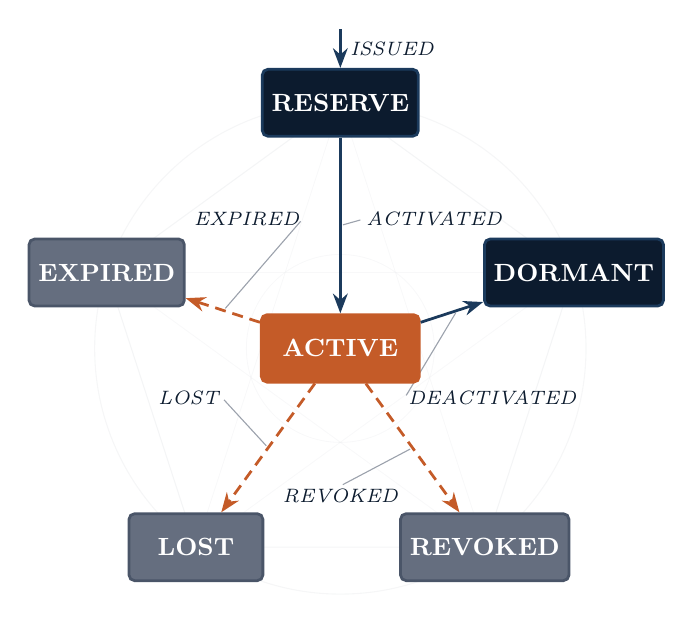
\begin{tikzpicture}[
  scale=0.78, font=\small,
  state/.style={
    draw=navymid, line width=1pt, rounded corners=2pt,
    minimum width=1.7cm, minimum height=0.85cm,
    fill=navydark, text=white, font=\bfseries\small,
    align=center,
  },
  centerstate/.style={
    draw=accent, line width=1.2pt, rounded corners=2pt,
    minimum width=2.0cm, minimum height=0.85cm,
    fill=accent, text=white, font=\bfseries\small,
    align=center,
  },
  termstate/.style={
    draw=steelgray, line width=1pt, rounded corners=2pt,
    minimum width=1.7cm, minimum height=0.85cm,
    fill=steelgray!85, text=white, font=\bfseries\small,
    align=center,
  },
  trans/.style={->, draw=navymid, line width=1pt, >={Stealth[length=2.5mm]}},
  termtrans/.style={->, draw=accent, line width=1pt, >={Stealth[length=2.5mm]}, dash pattern=on 4pt off 2.5pt},
  lbl/.style={
    font=\scriptsize\itshape\color{navydark},
    inner sep=1pt,
  },
  leader/.style={
    draw=steelgray, line width=0.4pt, opacity=0.55,
    shorten >=1pt, shorten <=1pt,
  },
]

% Background sacred geometry: pentagon + pentagram + circumscribed circle
\begin{scope}[on background layer]
  % Five vertices at 90, 162, 234, 306, 18 degrees (pentagon, top vertex)
  \coordinate (P1) at (90:4);   % top: RESERVE
  \coordinate (P2) at (162:4);  % upper-left: EXPIRED
  \coordinate (P3) at (234:4);  % lower-left: LOST
  \coordinate (P4) at (306:4);  % lower-right: REVOKED
  \coordinate (P5) at (18:4);   % upper-right: DORMANT
  % Pentagon outline
  \draw[steelgray, line width=0.4pt, opacity=0.06] (P1) -- (P2) -- (P3) -- (P4) -- (P5) -- cycle;
  % Pentagram (golden-ratio diagonals)
  \draw[steelgray, line width=0.3pt, opacity=0.04]
    (P1) -- (P3) -- (P5) -- (P2) -- (P4) -- cycle;
  % Circumscribed circle
  \draw[steelgray, line width=0.4pt, opacity=0.05] (0,0) circle (4);
  % Inner pentagon (formed by pentagram intersections)
  \draw[steelgray, line width=0.3pt, opacity=0.04] (0,0) circle (1.53);
\end{scope}

% States at pentagon vertices (narrowed boxes give labels room)
\node[state] (reserve)  at (90:4)  {RESERVE};
\node[termstate] (expired) at (162:4) {EXPIRED};
\node[termstate] (lost)    at (234:4) {LOST};
\node[termstate] (revoked) at (306:4) {REVOKED};
\node[state] (dormant)  at (18:4)  {DORMANT};

% ACTIVE at center
\node[centerstate] (active) at (0,0) {ACTIVE};

% Transitions: drawn first (without labels) so line styles are clean
% and continuous. Solid navymid for non-terminal, dashed accent for terminal.
\draw[trans] (reserve) -- (active);
\draw[trans] (active)  -- (dormant);
\draw[termtrans] (active) -- (revoked);
\draw[termtrans] (active) -- (lost);
\draw[termtrans] (active) -- (expired);

% Initial state arrow into RESERVE
\draw[trans] ($(reserve)+(0,1.2)$) -- (reserve) node[lbl, midway, right=2pt] {ISSUED};

% Labels: placed in the wedges between adjacent radial arrows, each
% with a thin leader line pointing to the midpoint of its associated
% transition arrow. This keeps labels in clear empty space, never
% overlapping arrow lines or destination state boxes, while a small
% connector makes the label-to-arrow association unambiguous.
%
% Each label sits in the wedge IMMEDIATELY clockwise of its arrow's
% direction, at the wedge bisector at radius 2.5. The five wedge
% bisectors are at 54°, 342°, 270°, 198°, 126°. Leader endpoints are
% the midpoints of each radial arrow at radius 2.0.

% Wedge bisector label coordinates and arrow midpoint coordinates.
% Labels positioned at radius 2.6 to clear all arrow lines and pulled
% to wedge bisectors so each sits squarely in its own zone. Leader
% endpoints at arrow midpoints (radius 2.0) provide unambiguous
% label-to-arrow association.
\coordinate (lblActivated)    at (54:2.6);
\coordinate (lblDeactivated)  at (342:2.6);
\coordinate (lblRevoked)      at (270:2.4);
\coordinate (lblLost)         at (198:2.6);
\coordinate (lblExpired)      at (126:2.6);

\coordinate (midActivated)    at (90:2.0);
\coordinate (midDeactivated)  at (18:2.0);
\coordinate (midRevoked)      at (306:2.0);
\coordinate (midLost)         at (234:2.0);
\coordinate (midExpired)      at (162:2.0);

% Labels first, named so leaders can terminate at label edges via
% TikZ's shape-aware path shortening (anchors at named node boundaries).
\node[lbl] (nodeActivated)   at (lblActivated)   {ACTIVATED};
\node[lbl] (nodeDeactivated) at (lblDeactivated) {DEACTIVATED};
\node[lbl] (nodeRevoked)     at (lblRevoked)     {REVOKED};
\node[lbl] (nodeLost)        at (lblLost)        {LOST};
\node[lbl] (nodeExpired)     at (lblExpired)     {EXPIRED};

% Leaders: from label boundary (TikZ auto-clips at node edge) to arrow
% midpoint with small offset back from arrow line.
\begin{scope}[on background layer]
  \draw[leader] (nodeActivated.west)   -- (midActivated);
  \draw[leader] (nodeDeactivated.west) -- (midDeactivated);
  \draw[leader] (nodeRevoked.north)    -- (midRevoked);
  \draw[leader] (nodeLost.east)        -- (midLost);
  \draw[leader] (nodeExpired.east)     -- (midExpired);
\end{scope}

\end{tikzpicture}

\caption{Token lifecycle state machine. \texttt{ACTIVE} at the center is the only operational state; the five surrounding states are reached by transitions from \texttt{ACTIVE} except \texttt{RESERVE}, which is the sole entry point from issuance. Solid arrows are non-terminal transitions; dashed arrows in accent are terminal (the token never returns from \texttt{REVOKED}, \texttt{LOST}, or \texttt{EXPIRED}). \texttt{DORMANT} is non-terminal in principle (audit access is preserved) but tokens never re-enter \texttt{ACTIVE} from \texttt{DORMANT}; succession runs through a fresh \texttt{RESERVE}-to-\texttt{ACTIVE} chain on the successor token, with \texttt{predecessor\_token\_id} carrying the lineage.}
\label{fig:state-machine}
\end{figure}

\subsection*{Production Enforcement of the State Machine}

The schema expresses three of the state machine's invariants directly: the domain of \texttt{status} is constrained by a \texttt{CHECK} clause that admits only the six legal values; the at-most-one-\texttt{ACTIVE}-per-individual invariant is enforced by the partial unique index on \texttt{individual\_id} where \texttt{status='ACTIVE'}; the requirement that every state change be audited is enforced operationally by pairing each \texttt{UPDATE IdentityToken} with a corresponding \texttt{INSERT INTO TokenLifecycleEvent} in the same transaction. These three are sufficient to prevent the most damaging illegal states.

The \textit{transitions} themselves are not directly expressible as schema-level constraints because SQL has no first-class concept of state-machine arrows. A production deployment would enforce them through one of three mechanisms. \textbf{Database triggers} on \entity{IdentityToken} can reject \texttt{UPDATE} statements whose \texttt{(OLD.status, NEW.status)} pair is not in the legal-transitions set; this is the strongest option because it guarantees enforcement regardless of which client connects to the database. \textbf{Stored procedures} that wrap each transition (\texttt{activate\_reserve}, \texttt{revoke\_token}, \texttt{record\_loss}) can be granted to application roles while direct \texttt{UPDATE} privileges on \entity{IdentityToken} are revoked; this is the most auditable option because every transition becomes a named, logged operation. \textbf{Application-layer enforcement} in the verifying service can mirror the state machine in code; this is the least defensible option in isolation, since a misconfigured second client can violate the invariants, but it is acceptable when paired with one of the database-level mechanisms. The recommendation is triggers for the hard edges (no return from terminal states) and stored procedures for the routine transitions, with the application layer treating both as opaque.

% ============================================================================
% APPENDIX B: INDEXING STRATEGY AND QUERY PLANS
% ============================================================================
% \newpage  (removed for compactness; let appendix flow)
\needspace{3\baselineskip}
\section{Indexing Strategy and Query-Plan Notes}
\label{app:indexing}

\begin{table}[H]
\centering
\footnotesize
\caption{Secondary indexes and the queries they support.}
\rowcolors{2}{tabstripe}{white}
\begin{tabularx}{\textwidth}{l l >{\RaggedRight\arraybackslash}X}
\toprule
\rowcolor{tabheader}
\thead{Index} & \thead{Cardinality} & \thead{Motivating Query / Access Pattern} \\
\midrule
\texttt{idx\_identitytoken\_individual} & High (1 per holder) & UC-7 history reconstruction; the partial unique constraint also benefits from this index for fast active-token lookup. \\
\texttt{idx\_identitytoken\_status} & Low (6 distinct values) & The \texttt{ActiveTokens} view scans tokens with \texttt{status='ACTIVE'} only; index used for filtering before join. \\
\texttt{idx\_verificationevent\_timestamp} & Very high & Capacity-planning queries (Q5), audit history retrieval (UC-7), and time-bounded subscription windows. \\
\texttt{idx\_verificationevent\_context} & Low (7 distinct values) & Per-context analytics (Q5); per-context fraud detection. \\
\texttt{idx\_tokenlifecycle\_token} & Moderate & Reconstructing a single token's lifecycle on demand (UC-4 reserve activation, UC-7 audit). \\
\bottomrule
\end{tabularx}
\end{table}

\subsection*{Notes on Query Plans}

Three of the six relational-algebra queries deserve specific attention:

\textbf{Query 1 (UC-7 banking history).} Filters \entity{VerificationEvent} on \texttt{outcome='SUCCESS'}, joins \entity{VerificationContext} on \texttt{context\_id}, and joins \entity{Individual} through \entity{IdentityToken} on \texttt{individual\_id}. The planner should first restrict by \texttt{outcome} (column not currently indexed; \textbf{candidate for an additional index} if banking-history queries become frequent), then use \texttt{idx\_verificationevent\_context} for the context join, then nested-loop-join through the token to the individual. Estimated cost: $O(N_v \cdot \log N_t)$ where $N_v$ is verification-event count and $N_t$ is token count.

\textbf{Query 5 (verification volume by context).} Pure aggregation over \entity{VerificationEvent} grouped by \texttt{context\_id}. The planner uses \texttt{idx\_verificationevent\_context} to drive a hash-aggregate. With 7 distinct context values, the aggregate is bounded; the join to \entity{VerificationContext} for human-readable labels is a 7-row lookup. Cost: $O(N_v)$.

\textbf{Query 6 (succession lineage).} Self-join on \entity{IdentityToken} via the nullable \texttt{predecessor\_token\_id}. The planner uses the primary key on \texttt{token\_id} for the inner side. A future enhancement is a dedicated \texttt{idx\_identitytoken\_predecessor} index; with the current sample-data size it is unnecessary, but a production deployment with hundreds of millions of tokens should add it.

\subsection*{Partitioning Recommendation (Future Work)}

\entity{VerificationEvent} is the only table that grows without bound in normal operation. A national deployment would generate on the order of $10^8$ to $10^9$ rows per year. Two partitioning strategies are candidates:

\begin{itemize}
  \item \textbf{Range partitioning on \texttt{event\_timestamp}}, monthly. Old partitions can be archived to cold storage and detached from the live table without touching the rest of the schema. This is the recommended primary strategy.
  \item \textbf{List partitioning on \texttt{context\_id}}, secondary. Verification volume is unlikely to be uniform across contexts (banking dominates), so context-list partitioning helps with parallel-scan performance for context-specific queries.
\end{itemize}

PostgreSQL 14+ supports both. A composite partitioning scheme (range on timestamp, then list on context within each monthly partition) is feasible but not recommended initially.

% ============================================================================
% APPENDIX C: COMPARATIVE ANALYSIS
% ============================================================================
% \newpage  (removed for compactness; let appendix flow)
\section{Existing National Identity Systems}
\label{app:comparison}

The Identity Token System is not the first attempt at a unified digital credential. Five existing systems represent the design space the present schema must situate itself within. Each is summarized below, followed by a comparative table.

\textbf{A federated national eID with a data-exchange backbone.} The most mature national digital-identity infrastructure in production issues every resident a state-issued chip card with two PKI key pairs (authentication and signing) under a state-operated certificate authority. Behind the card sits a federated data-exchange backbone that lets agencies verify identity and exchange data without centralizing it. The architecture has operated for over two decades and is the closest live analogue to the present design, but its PKI is not post-quantum.

\textbf{ISO 18013-5 Mobile Driver's License (mDL).} An international standard for mobile-phone-based driver's licenses, finalized in 2021 and adopted by several US states (Arizona, Iowa, Maryland, Mississippi, Oklahoma, Utah, Colorado, others) plus Australia and Argentina. The mDL standard supports selective disclosure but stores the credential on a phone, not a hardware token, and does not address replacement contexts beyond driving authority. Quantum resistance is a roadmap item.

\textbf{India Aadhaar.} The world's largest biometric identification system, with over 1.3 billion enrollments. Aadhaar centralizes biometric templates (fingerprint and iris) in a national database (the Central Identities Data Repository), which is the precise architectural choice the present design rejects. Verification is done by sending biometric samples to the centralized database, which returns a yes/no response. The system has been the subject of substantial constitutional litigation in India; the 2018 Puttaswamy decision restricted but did not abolish it.

\textbf{EU eIDAS 2.0 / European Digital Identity Wallet.} The EU's 2024 regulation establishing a federated digital-identity framework across all 27 member states, with the European Digital Identity Wallet (EUDI Wallet) as the user-facing artifact. Architecturally federated rather than centralized: each member state issues credentials, and the wallet aggregates them. Selective disclosure is mandated. Post-quantum migration is in roadmap discussions but not yet specified.

\textbf{W3C Verifiable Credentials and Decentralized Identifiers.} A standards stack rather than a deployment: \texttt{did:} URI scheme, JSON-LD credential format, BBS+ signatures for selective disclosure. Adopted by Microsoft Entra Verified ID, IBM Digital Credentials, and several blockchain projects. The standards are issuer-agnostic; the present design's optional \entity{BlockchainAnchor} entity is the bridge to this ecosystem.

\begin{table}[H]
\centering
\footnotesize
\caption{Comparison of identity-system architectures.}
\setlength{\tabcolsep}{4pt}
\renewcommand{\arraystretch}{1.15}
\rowcolors{2}{tabstripe}{white}
\begin{tabularx}{\textwidth}{>{\bfseries\RaggedRight\arraybackslash}p{1.4in} >{\RaggedRight\arraybackslash}p{1.05in} >{\RaggedRight\arraybackslash}p{0.95in} >{\RaggedRight\arraybackslash}p{0.95in} >{\RaggedRight\arraybackslash}X}
\toprule
\rowcolor{tabheader}
\thead{System} & \thead{Trust Model} & \thead{Biometric} & \thead{Revocation} & \thead{Post-Quantum} \\
\midrule
Federated national eID  & Federated state CA & Optional, on-device & OCSP / CRL & Classical (RSA, ECDSA) \\
ISO 18013-5 mDL       & Issuer-signed & On-device & Status list & Classical; PQ on roadmap \\
India Aadhaar         & Centralized (UIDAI) & Required; central template & Lock flag & Classical \\
EU eIDAS 2.0 EUDI     & Federated, per-MS issuers & Optional, on-device & Status list & Classical; PQ planned \\
W3C VC / DID stack    & Decentralized & N/A (out of scope) & Revocation registry & PQ-capable (BBS+) \\
\midrule
\rowcolor{tabstripe}
\textbf{Identity Token (this work)} & \textbf{Federated + DID anchor} & \textbf{On-device only} & \textbf{\entity{RevocationList} + \texttt{status}} & \textbf{Native PQ (ML-DSA, SLH-DSA)} \\
\bottomrule
\end{tabularx}
\end{table}

\subsection*{Where the Present Schema Sits}

The Identity Token System borrows the federated trust model from a mature federated national eID and eIDAS, the on-device biometric model from mDL, the optional decentralized-identifier anchoring from W3C VC, and the post-quantum signature primitives from NIST. It rejects Aadhaar's centralized-biometric model and the classical-cryptography posture of every other system (NIST having formally finalized post-quantum standards in August 2024). The deliberate distinguishing feature is the \texttt{disclosure\_level} column on \entity{VerificationEvent}: none of the five comparison systems carries a comparable schema-level mechanism for preventing the verification log from functioning as a surveillance database. mDL and EUDI permit selective disclosure at the protocol level but record verifications at full granularity in the verifier's logs; the present schema makes the disclosure level a property of the persisted record itself.

\subsection*{Patterns Across the Field}

Reading the five comparison systems together reveals two convergences and one open question. \textbf{Federation has won.} Aadhaar is the only large-scale centralized system in the comparison; every other architecture (the federated national eID, mDL, eIDAS 2.0, W3C VC) federates issuance across multiple authorities. The post-Snowden, post-Equifax design environment treats centralized biometric repositories as inherently untenable, regardless of operator intent. \textbf{On-device biometric handling has won.} mDL, eIDAS 2.0, and the present design all keep biometric templates in the holder's device and reduce verification to a yes/no signal sent to the verifier. Aadhaar's centralized template repository is the architectural outlier even within India's own roadmap discussions. The open question is \textbf{post-quantum migration}. That national eID is on classical cryptography with no announced migration plan; mDL has post-quantum on its roadmap but no schedule; eIDAS 2.0 has it in active discussion but no specified target date; W3C VC supports BBS+ signatures, which are PQ-capable but not PQ-mandatory. Polaris's choice to make post-quantum primitives the only signing option for new tokens is the outlier in 2026; by 2030 it should be the median.

% ============================================================================
% APPENDIX D: THREAT MODEL
% ============================================================================
% \newpage  (removed for compactness; let appendix flow)
\section{Threat Model (STRIDE)}
\label{app:threat-model}

STRIDE is Microsoft's threat-classification framework: \textbf{S}poofing, \textbf{T}ampering, \textbf{R}epudiation, \textbf{I}nformation disclosure, \textbf{D}enial of service, \textbf{E}levation of privilege. It is the right framework for this analysis because each of its six categories maps directly to a class of database-layer attack, and the framework is exhaustive over the threats that the schema itself can defend against. Threat models scoped at the application or network layer (PASTA, OCTAVE, attack trees) would miss the schema-level mitigations this design relies on; STRIDE is structured to surface exactly them.

The analysis below scopes the threat model to the database layer. This is a deliberate restriction: the schema can guarantee what it is queryable for and what it refuses to store, but it cannot guarantee what happens before data arrives at the database (compelled biometric presentation, issuer-key compromise) or what happens after data leaves it (exfiltration through a privileged client). The three categories of threat outside the schema's reach are enumerated in the subsection that follows the table. The \textit{Schema-Level Mitigation (and Residual Risk)} column is therefore the operative one: it states what the schema does and, where present, what it does not do even when it does its job correctly.

\begin{table}[H]
\centering
\scriptsize
\caption{STRIDE analysis of the Identity Token System schema.}
\setlength{\tabcolsep}{4pt}
\renewcommand{\arraystretch}{1.05}
\rowcolors{2}{tabstripe}{white}
\begin{tabularx}{\textwidth}{>{\bfseries}p{1.35in} >{\RaggedRight\arraybackslash}X >{\RaggedRight\arraybackslash}X}
\toprule
\rowcolor{tabheader}
\thead{Category} & \thead{Threat} & \thead{Schema-Level Mitigation (and Residual Risk)} \\
\midrule
Spoofing & Adversary presents a stolen or counterfeit token to a verifier. & On-device biometric binding gates token use; \texttt{biometric\_binding\_type} on \entity{IdentityToken} records the method. Template never enters the database. Residual risk: compelled biometric presentation. \\
Tampering & Adversary modifies a token's signature, status, or permissions. & Tokens are signed under a NIST PQ algorithm (\texttt{ML-DSA}, \texttt{SLH-DSA}) recorded in \entity{CryptographicAlgorithm}; database-level changes require write access addressed by deployment hardening. \\
Repudiation & A verifier or issuer denies an action they performed. & \entity{TokenLifecycleEvent} is an append-only audit trail with \texttt{actor\_agency\_id}; \entity{VerificationEvent} records \texttt{requesting\_agency\_id}. The append-only invariant is by convention and tooling. \\
Information Disclosure & Verification log becomes a surveillance database, or biometric templates are exfiltrated. & \texttt{disclosure\_level} on \entity{VerificationEvent} controls persistence: \texttt{ZERO\_KNOWLEDGE} stores only a commitment; \texttt{SELECTIVE} discloses specified attributes; \texttt{FULL} is restricted to warrant-authorized verification. Templates never stored centrally. \\
Denial of Service & Adversary overwhelms the verification layer or relies on stale revocation data. & Indexes (Appendix~\ref{app:indexing}) keep single-row lookups at $O(\log N)$; rate limiting is deferred to deployment. \entity{RevocationList} carries \texttt{published\_location} for verifier freshness checks. \\
Elevation of Privilege & An agency issues or verifies under an algorithm it is not authorized to use. & \entity{AgencyAlgorithmAuth} enforces \texttt{ISSUE} / \texttt{VERIFY} / \texttt{BOTH} per (agency, algorithm) pair; \entity{Agency} carries \texttt{authorization\_level} (1--5) for coarse-grained policy. \\
\bottomrule
\end{tabularx}
\end{table}

\subsection*{Threats Outside the Schema's Reach}

Three categories of threat the database layer cannot mitigate. \textit{Compelled biometric presentation:} an actor with physical access can compel fingerprint, iris, or face presentation; the schema cannot distinguish coerced from voluntary use, and hardware-level features (duress codes, attestation delays) are needed. \textit{Issuer compromise:} if an issuing agency's signing keys are compromised, every token it issued is suspect; mitigation requires cryptographic diversity across issuers and out-of-band attestation channels. \textit{Cryptanalytic advance:} should ML-DSA or SLH-DSA be broken before scheduled migration, the entire token population is at risk; \texttt{deprecation\_date} enables proactive planning, but multi-signature transitional states are not yet modeled (noted in Limitations).

% ============================================================================
% APPENDIX E: THE SUBSTRATE LAYER
% ============================================================================
% \newpage  (removed for compactness; let appendix flow)
\section{Why Identity Cannot Outrun Its Primitives}
\label{app:substrate}

Section~\ref{subsec:pq-day-one} justified treating post-quantum signing as the schema's operating regime through Mosca's inequality and the time horizon of identity data. This appendix formalizes the deeper architectural argument: cryptographic primitives constitute the \textit{substrate} of digital sovereignty, and every higher-level property of an identity system is derivative of the primitives it sits on top of. Identity infrastructure is conventionally drawn as a layered stack: hardware roots of trust, cryptographic primitives, authenticated communications, identity and authentication, data sovereignty, and at the top, algorithmic governance. The schema sits at the identity and authentication layer. Every higher-level property it implements (authenticity of signed credentials, integrity of audit trails, binding of biometric attestations, validity of zero-knowledge proofs) is derivative of properties at the cryptographic substrate two layers below. Change the primitive and the property changes; compromise the primitive and the property has no referent. The visible operations of an identity system are not buildings on a foundation but emanations of the substrate, downstream of a one-way causal descent through every authenticated, signed, or attested operation in the stack.

Classical public-key cryptography rests on factorization and discrete-log hardness. Shor's algorithm (1994) demonstrated that a sufficiently large quantum computer solves both in polynomial time: the hardness assumption is not weakened, it is annihilated. Two consequences follow from this single mathematical fact, and they apply to identity infrastructure asymmetrically. \textbf{Signatures}: every credential signed today under ECDSA or RSA can be \textit{forged} once Shor-capable hardware reconstructs the issuing key, which means the binding between a biometric anchor and a holder's legal identity becomes asserted by whichever adversary recovers the key, not only by the original issuer. \textbf{Encrypted material}: any ciphertext intercepted today and stored under classical key exchange (TLS handshakes, sealed identity proofs, archived authentication transcripts) sits in a latent pre-collapse state, decryptable when the substrate transitions; harvest-now-decrypt-later is the operational name for this pattern. The transition is not an attack but a phase transition: the cryptographic past does not become vulnerable when a cryptographically relevant quantum computer enters service, it becomes \textit{determined}. The schema's signed bindings and any associated wire-protocol transcripts are both implicated.

Three implications follow. \textbf{First}, the schema cannot be built defensively against a post-rendering substrate: the transition is discontinuous, and no schema-level mechanism recovers what is lost when a primitive becomes meaningless. The correct response is to architect for the post-rendering substrate from the start, which is what this design does by refusing to issue new tokens under classical algorithms. \textbf{Second}, sovereignty at the database layer is derivative of sovereignty at the primitive layer; a schema implementing the strongest privacy controls over signatures from an adversary-authored algorithm produces compliance, not sovereignty. The commitment to NIST-finalized primitives (FIPS 203, 204, 205) is a sovereignty stance, not a technical preference. \textbf{Third}, the database layer is not the only layer at which an identity system can fail; the human substrate (credentialed operators) and the operational substrate sit outside the relational schema's scope. The schema can refuse to amplify their failure modes but cannot substitute for human-level and policy-level controls.

% ============================================================================
% APPENDIX F: BEYOND BIOMETRIC BINDING
% ============================================================================
\section{Beyond Biometric Binding}
\label{app:beyond-biometric}

The current schema records biometric binding through the \texttt{biometric\_binding\_type} column on \entity{IdentityToken}, which admits four values: \texttt{NONE}, \texttt{FINGERPRINT}, \texttt{FACE}, and \texttt{IRIS}. This is the strongest binding mechanism that production hardware can deliver in 2026. It is not the strongest binding mechanism that is possible in principle. This appendix sketches two extensions of the binding model that the schema would need to accommodate as the underlying hardware advances: \textbf{genomic binding} as a near-term hardware extension, and \textbf{quantum-observer binding} as a far-future architecture that closes the binding chain at the only link no adversary can copy.

\subsection*{F.1\quad Genomic Binding (Near-Term Hardware Extension)}

A genomic binding extension would add \texttt{GENOMIC} to the \texttt{biometric\_binding\_type} domain and introduce a \entity{GenomicCommitment} entity holding zero-knowledge proofs of uniqueness over the holder's genome. The raw genome would never enter the database; only homomorphic commitments and ZK proofs would. The owner's secure enclave would hold the sequence locally and produce per-verification proofs. A human genome carries roughly $3 \times 10^9$ base pairs, of which $\sim 4{\text{--}}5 \times 10^6$ vary between individuals --- more than sufficient entropy to defeat any forgery attack at scale.

The architectural problem is that \textbf{genomic data can still be stolen}. The threat surface is well-documented: consumer-genomics breaches (23andMe, October 2023, $\sim$7M profiles), surreptitious public-space collection, state-level exfiltration from medical or research databases, and synthesis attacks reconstructing the profile from partial-relative data. Once the profile is in adversarial hands, the binding is broken: the owner's body is no longer the only entity that can produce a valid proof. This is the fundamental ceiling of any binding tied to \textit{biological data} --- the data is copyable.

\subsection*{F.2\quad Quantum-Observer Binding (Speculative)}

The next horizon abandons binding to biological \textit{data} and binds instead to the \textit{act} of observation. Measurement in quantum mechanics is not passive; the resulting collapse is irreproducible by anyone who did not perform it. The cryptographic realization uses quantum entanglement: the token's authenticating key material is prepared as a Bell-type entangled state, half held in the token's secure quantum register and half projected through a brain-computer interface tuned to the owner's neural quantum signature. The state cannot be duplicated (no-cloning theorem) and cannot be shared (monogamy of entanglement). When the owner directs attention through the BCI, the measurement collapses the entangled pair into the correct decryption key for that authentication moment; any other observer's measurement collapses it into noise. Under the contested but seriously-discussed Orch-OR hypothesis (Penrose-Hameroff), quantum-coherent processes in microtubular cytoskeletons make the collapse pattern specific to a brain's connectome --- a fingerprint no apparatus simulates without instantiating an equivalent neural architecture.

None of this is engineered in 2026; the architecture is a research direction. Returning to the threat model in Appendix~\ref{app:threat-model}: of the three residual risks, quantum-observer binding directly addresses compelled biometric presentation. Under stress the neural signature shifts and the state decoheres without yielding the key; the binding is not merely \textit{tied to} the holder, it \textit{is} the holder. The three generations (biometric, genomic, quantum-observer) form a nested progression that the present schema would resolve through a hypothetical \texttt{TokenBinding} junction table replacing the current scalar \texttt{biometric\_binding\_type} column; everything else is hardware, physics, and time.

\end{document}
